%%%%%%%%%%%%%%%%%%%%%%%%%%%%%%%%%%%%%%%%%%%%%%%%%%%%%%%%%%%%
%%% ELIFE ARTICLE TEMPLATE
%%%%%%%%%%%%%%%%%%%%%%%%%%%%%%%%%%%%%%%%%%%%%%%%%%%%%%%%%%%%
%%% PREAMBLE 
\documentclass[9pt,lineno]{elife}

\usepackage[export]{adjustbox}
\usepackage{lscape}
\usepackage{afterpage}
\usepackage{hyperref}
\hypersetup{
    colorlinks=true,
    linkcolor=blue,
    filecolor=magenta,      
    urlcolor=cyan,
}

\newcommand{\sgcomment}[1]{\textcolor{blue}{SG: #1}}
\newcommand{\luke}[1]{\textcolor{blue}{Luke: #1}}
\newcommand{\todo}[1]{\textcolor{blue}{*#1*}}
\newcommand{\alex}[1]{\textcolor{red}{Alex: #1}}
%%%%%%%%%%%%%%%%%%%%%%%%%%%%%%%%%%%%%%%%%%%%%%%%%%%%%%%%%%%%
%%% ARTICLE SETUP
%%%%%%%%%%%%%%%%%%%%%%%%%%%%%%%%%%%%%%%%%%%%%%%%%%%%%%%%%%%%
\title{Legacy Data Confounds Modern Genomics Studies}

\author[1,2]{Luke Anderson-Trocm\'e}
\author[1,2]{Mathieu Bourgey}
\author[1,2]{Rick Farouni}
\author[3]{Fumihiko Matsuda}
\author[3]{Yoichiro Kamatani}
\author[1,2]{Simon Gravel}

\affil[1]{Department of Human Genetics, McGill University, Montreal, QC H3A 0G1, Canada}
\affil[2]{McGill University and Genome Quebec Innovation Centre, Montreal, QC H3A 0G1, Canada}
\affil[3]{Center for Genomic Medicine, Graduate School of Medicine, Kyoto University, Kyoto 606-8501, Japan}
\corr{simon.gravel@mcgill.ca}{SG}

%%%%%%%%%%%%%%%%%%%%%%%%%%%%%%%%%%%%%%%%%%%%%%%%%%%%%%%%%%%%
%%% ARTICLE START
%%%%%%%%%%%%%%%%%%%%%%%%%%%%%%%%%%%%%%%%%%%%%%%%%%%%%%%%%%%%

\begin{document}

\maketitle
\begin{abstract}
Recent reports have identified differences in the mutational spectra across human populations. While some of these reports have been replicated in other cohorts, most have been reported in the 1000 Genomes project data. While investigating an intriguing putative population stratification within the Japanese population, we identified a previously unreported batch effect leading to spurious mutation calls in the 1000 Genomes Project data and to the apparent population stratification. Because the 1000 Genomes data is used extensively, we find that the spurious calls also lead to incorrect imputation by leading imputation servers and suspicious GWAS associations. Lower-quality data from the early phases of the 1000 Genomes project thus contaminates modern studies in hidden ways, and a community effort may be required to remove or upgrade such legacy sequencing data from reference databases. 
\end{abstract}

\section{Introduction}
		
\subsection{Reference Cohorts}			

The last 5 years have seen a drastic increase in the amount and quality of human genome sequence data. 
Hapmap \cite{HapMap2005}, the 1000 Genomes Project \cite{1000GenomesProjectConsortium2010,The1000GenomesProjectConsortium2012}, and the Simons Diversity project \cite{Mallick2016}, for example, have made thousands of genomes publicly available for population and medical genetic analyses. 
Many more genomes are available indirectly through servers providing imputation services \cite{ProfJonathanMarchiniProfGoncaloAbecasisProfRichardDurbin2014} or summary statistics for variant frequency estimation \cite{Lek2016}.

Because of the extraordinary value of freely available data, this early data from the 1kGP is still widely used as a reference panel for imputation, allele frequency estimations and to answer a wide range of medical and evolutionary questions. However, the first sequenced genomes in the 1000 Genomes project (1kGP), for example, were sequenced 10 years ago. Since then, sequencing platforms have rapidly improved. The second phase of the 1kGP describe multiple technological and analytical improvements over its earlier phases \cite{}. This led to heterogeneous sample preparations and data quality for many of the samples included in the dataset.

Even though it is intuitively clear that such batch effects have the potential to confound analyses, the usefulness and ubiquity of the 1kGP data makes such issues particularly insidious.   This raises the question of whether and how such legacy data should be included in contemporary analyses alongside more recent cohorts. 
Here we point out how large and previously unreported batch effects in the early phases of the 1kGP that still lead to incorrect genetic conclusions through population genetic analyses and indirect use through prominent imputation servers.  

\subsection{Motivations}

Different mutagenic processes preferentially affect different DNA motifs. Certain mutagens in tobacco smoke, for example, have been shown to preferentially bind to certain genomic motifs leading to an excess of G to T transversions \cite{Pleasance2010}. Thus, exposure of populations to different mutational processes can be inferred by considering the DNA context of polymorphism in search of `signatures' of different mutational processes\cite{Pleasance2010}. 
Such genome wide mutational signatures have been used as a diagnostic tool for cancers \cite{Pleasance2010,Shiraishi2015a}.

%While certain mutagens have very distinct mutational signatures, others are more subtle and difficult to identify because they tend to occur less frequently and with less genomic specificity \cite{Pleasance2010}.
%Large cohorts have recently become available to increase statistical power to resolve some of these finer scale mutational signatures.

Differences in mutational signatures across human populations have recently been reported.
In 2015, Harris reported 50\% more TCC ${\rightarrow}$ TTC mutations in European populations compared to African populations; this was replicated in a different cohort in 2017 \cite{Harris2015a}. 

Strong population enrichments of a mutational signature suggests important genetic or environmental differences in the history of each population \cite{Harris2015a}. 
Harris and Pritchard further identified distinct mutational spectra across a range of populations \cite{Harris2017a}, which were further studied in \cite{Voight}
 
 In particular, both studies  identified a heterogeneous mutational signature within 1000 Genomes Japanese individuals.
This heterogeneity is intriguing because differences in mutational signatures accumulate over many generations.
A systematic difference among the Japanese population would suggest sustained environmental or genetic differences across sub-populations within Japan with little to no gene flow.
We therefore decided to follow up on this observation, by using a newly sequenced dataset \sgcomment{description of cohort.}

While we were unable to reproduce the heterogeneity among the Japanese population, we could trace back the source of the discrepancy to a batch effect in the 1kGP data that we were not previously aware of.
We also found that this batch effect led to spurious results in a additional recent publications as a consequence of biased imputation. 

The results section is organized as follows:
First, we describe the observed discrepancies within and between studies. We then identify the technical covariates that strongly correlate with the discordant values, and describe the distribution of such covariates across phases and populations of the 1kGP.    
Next, we identify lists of SNPs from the 1kGP whose validity is highly debatable, and show that major imputation servers impute the dubious SNPs.  
Even though these SNPs are likely technical artifacts, we two recent studies report such SNPs as genome-wide significant hits.   

Fortunately, the main conclusions of most of the affected studies remain supported by other data. Yet this begs the question: When should we retire legacy reference data?

\begin{figure}
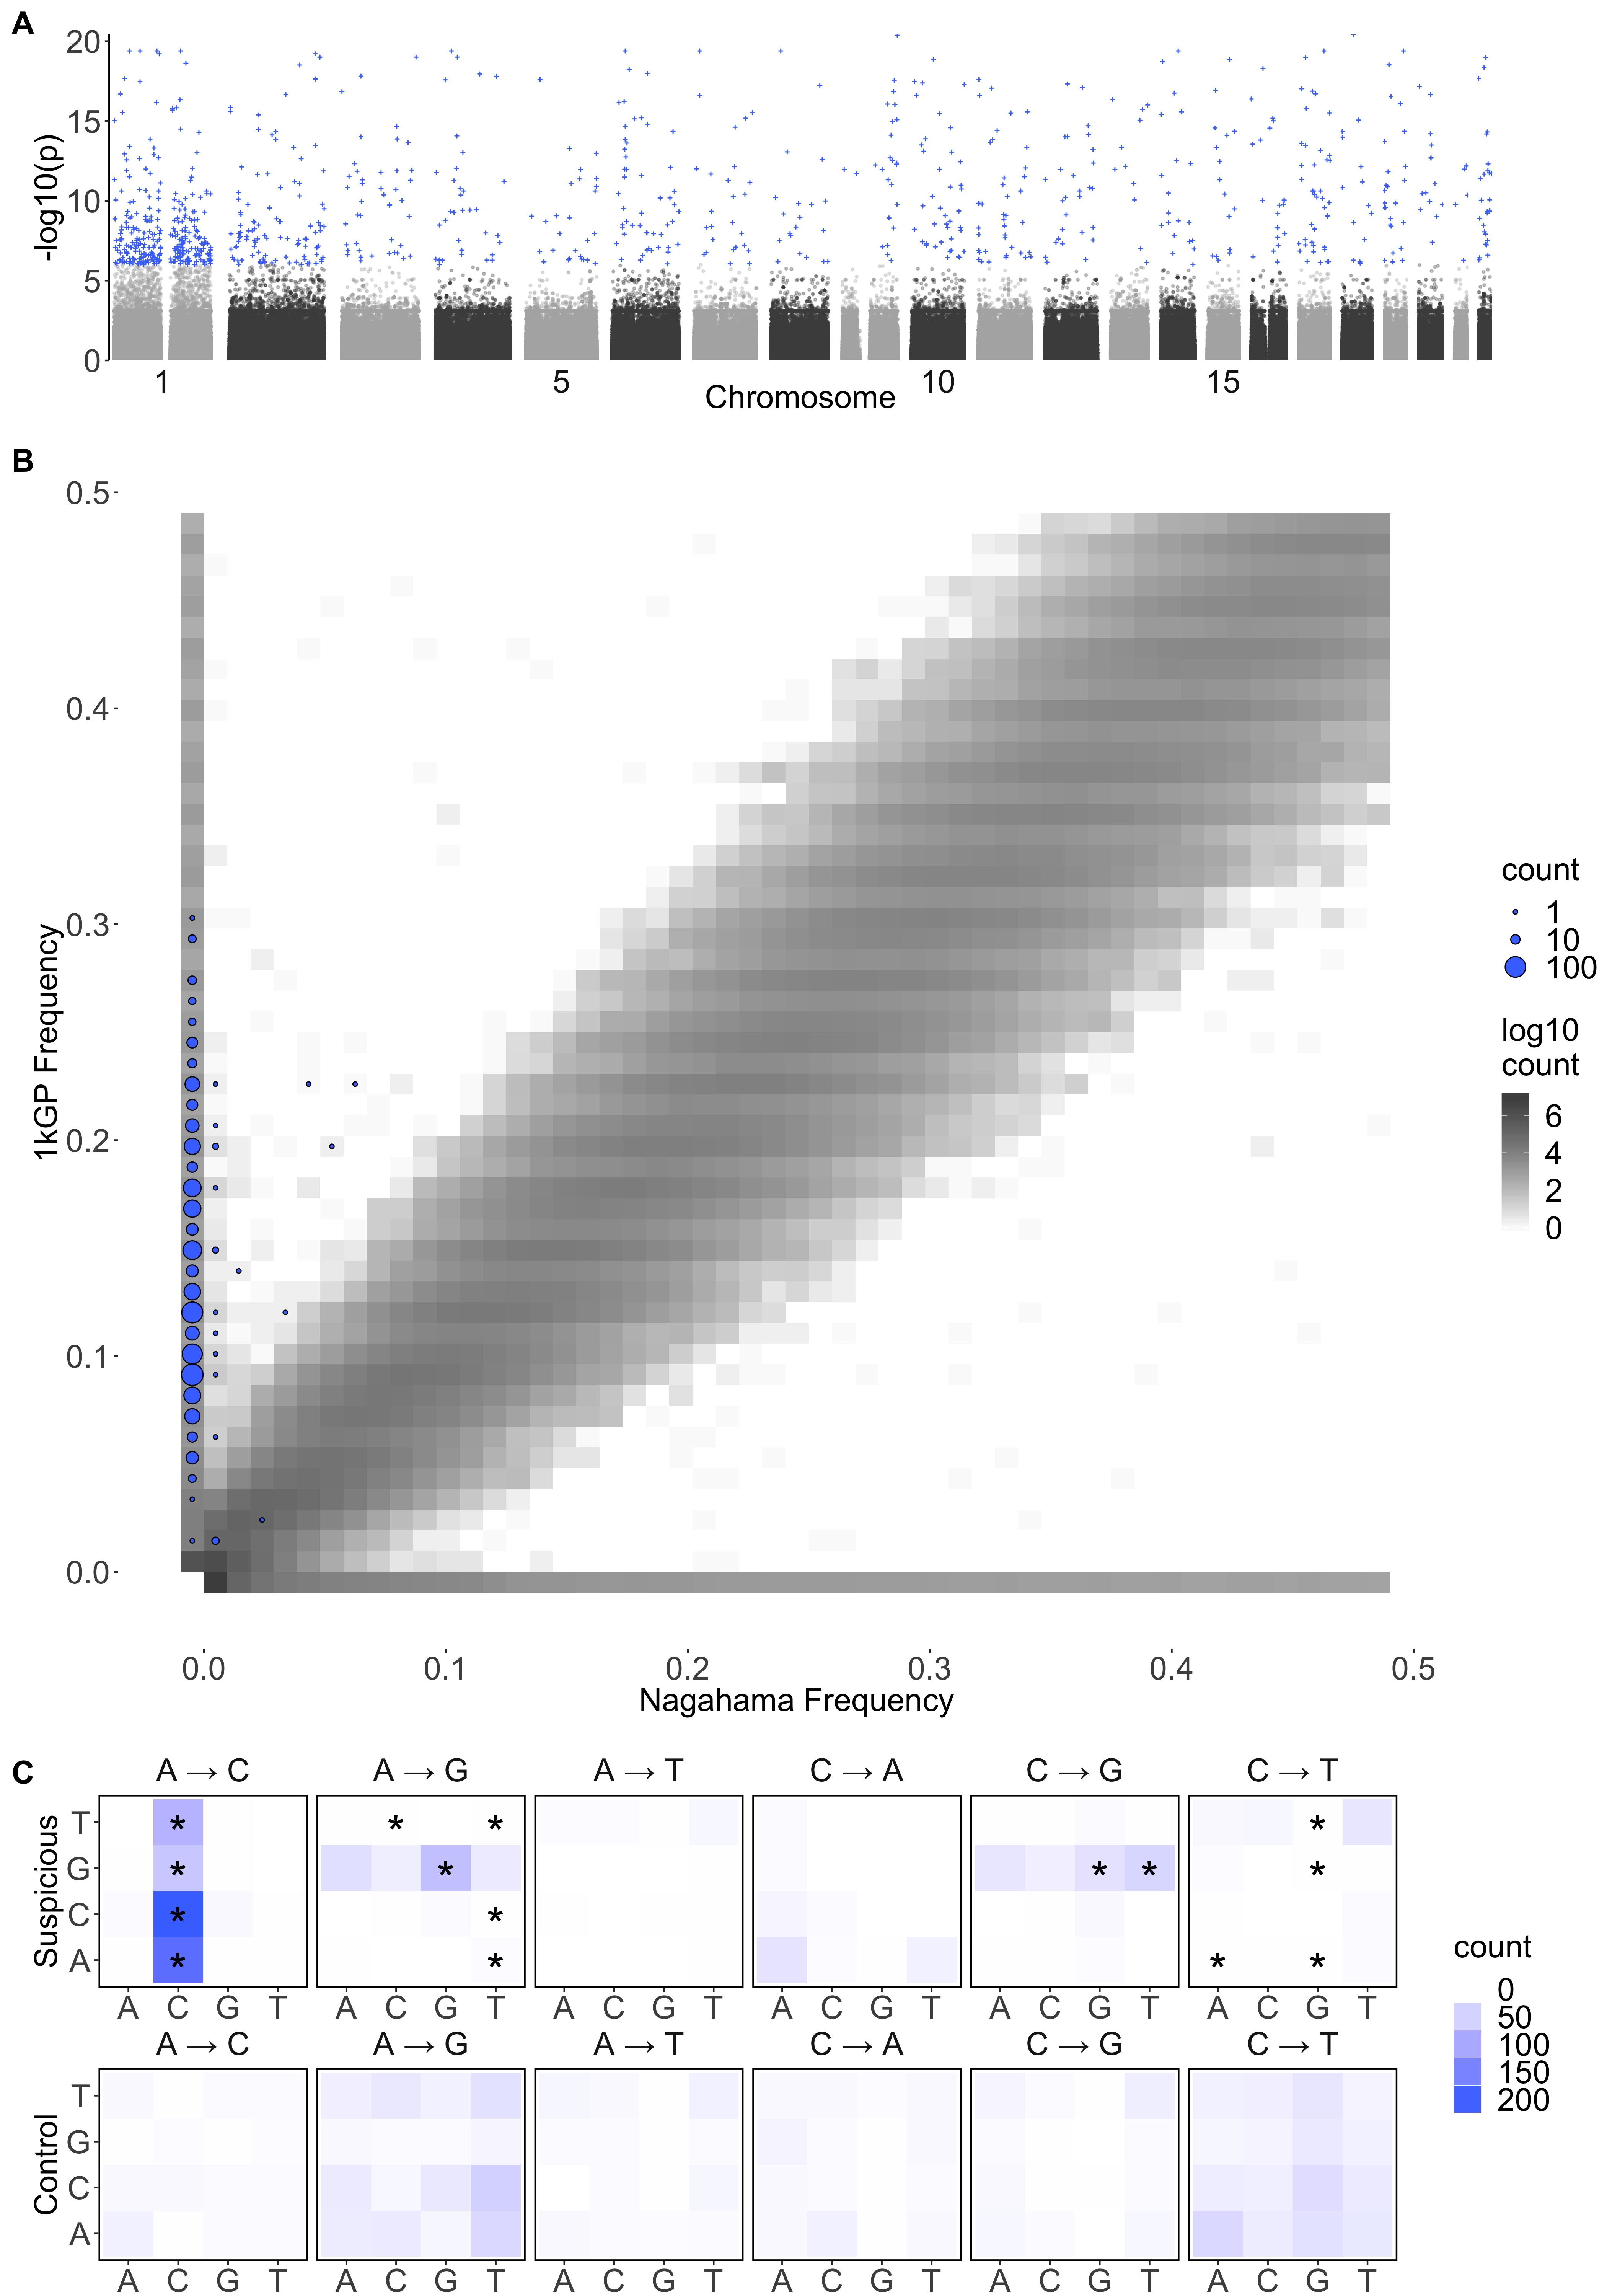
\includegraphics[width=\hsize,keepaspectratio]{./Figures/Figure1.jpg}
\caption{
\textbf{A} 
Mutation spectrum of the 1034 variants that reached a genome wide significance with a p value less than $p < 10^{-6}$  in a GWAS of sequencing quality. 
There majority of the variants with significant associations to quality have the *AC${\rightarrow}$*CC mutational pattern. There is also an slight enrichment in GA*${\rightarrow}$GG* and GC*${\rightarrow}$GG* mutations. These three enrichments can be summarized as G**${\rightarrow}$GG*. (note: the reverse complement of *AC${\rightarrow}$*CC is GT*${\rightarrow}$GG*)
\textbf{B} 
Joint frequency spectrum plot of the Japanese from the 1kGP and a more recent Nagahama dataset.
Crosses ( + ) are variants that reached genome wide significance in a GWAS of sequencing quality. 
The histogram on the left of the plot is the distribution of significant variants. 
\textbf{C} 
Genome wide association of the average quality of mapped bases for the 104 Japanese individuals included in the 1kGP. This GWAS identified $587\ \  p < 10^{-8}$ and $1034\ \ p < 10^{-6}$ SNPs that were associated to the average quality of SNPs mapped for an individual
The same analysis was performed independently for each of the populations in the 1kGP. }
 \label{SFS}
\end{figure}

			\section{Results}
	\subsection{A peculiar mutational signature in Japan}			
	
Harris and Pritchard reported an excess of a 3-mer *AC${\rightarrow}$*CC mutational pattern in a portion of the Japanese individuals in the 1kGP.\cite{Harris2015a}
While trying to follow up on this observations in a larger and more recent Japanese cohort, we did not find this particular signature.
However, when comparing the allele frequencies between the Japanese individuals from the 1kGP and this larger dataset, we observed an unusually large number of single nucleotide polymorphisms (SNPs) private to one of the two groups.
This is unexpected given the similarity of the two populations, and suggests a technical difference rather than a population structure effect. 
Moreover, these mismatches were maintained after filtering for low-quality regions of the human genome and standard metrics such as Hardy-Weinberg equilibrium.
Low frequency variants have little power to detect Hardy-Weinberg disequilibrium, in essence we would not expect any homozygous alternates for low frequency variants. 

When mismatch sites were removed from the 1kGP data, the  *AC${\rightarrow}$*CC signal disappears (Figure \ref{SFS}).
Regressions against different individual-level quality metrics provided by the 1kGP revealed that mean quality per mapped base pair per individual was an excellent correlate with prevalence of the  *AC${\rightarrow}$*CC mutational signature in 1kGP:
Individuals with low mapping quality show elevated rates of the signature (see Supplementary Figure \ref{PC1_Correlation}).
Thus sequences with low quality harbour mutations that reproduce poorly across studies and exhibit a particular mutational signature. 

To identify SNPs that are likely to reproduce poorly across cohorts (without having access to a second cohort), we performed a reverse genome-wide association study (GWAS) in the JPT for SNPs that correlate strongly with low quality (Figure \ref{SFS}).
Whereas the majority of GWAS use linear regression predicting a phenotype based on genotype, we are looking for loci where the genotypes are predictable based on the data quality scores.
This approach identifies 587 SNPs with $p < 10^{-8}$ and 1034 SNPs with $ p < 10^{-6}$.
While identifying putative low-quality SNPs to exclude, using a higher $p$-value threshold increases the stringency of the filtering (i.e., excluding SNPs with $ p < 10^{-6}$ is more stringent than excluding SNPS with $p < 10^{-8}$). 
The variants that are associated to the quality of mapped bases have an enrichment in *AC${\rightarrow}$*CC mutations, GA*${\rightarrow}$GG*, and GC*${\rightarrow}$GG* mutations.
These three enrichments can be summarized as an excess of G**${\rightarrow}$GG* in low-mapping quality individuals.

Thus this mutational signal is heavily enriched in GWAS suspicious SNPs, but residual signal remains in non-significant SNPs, presumably because many rare alleles found in individuals with low-quality data remain unidentifiable using association techniques. 

%For this reason, the heterogeneously distributed signal persisted in the 1kGP Japanese even after filtering the variants that were significantly associated to quality. 
The removal of individuals with average mapping quality below 30 successfully removes the *AC${\rightarrow}$*CC signal, however other signals identified by Harris and Pritchard appear unchanged. 
For population genetic analyses, the removal of individuals with low quality sequence data appears preferable to filtering positions. 

	\subsection{Sequencing quality over time}
The results of the logistic regression GWAS performed on the Japanese from the 1kGP lead us to consider whether any other populations in the 1kGP also had similar issues with data quality.
The average quality of sequencing data of individuals over time shows that the sequencing done in the early phases of the 1kGP was more variable and overall tended to include lower quality sequencing data (Figure \ref{MapQual}).
This variability could be as a result of fluctuating sequence platform protocols or variation between sequencing centres.
There were a number of protocols used to prepare the samples for sequencing, as well as a number of sequencing technologies used over the course of the data production.
By 2011, older sequencing technologies are phased out, and method development solidify, which coincides with the sequencing quality levelling off.
It's clear that there are many covariates that could be used to identify spurious sites like sequencing date, sequencing technology or even the sequencing centre. 
However, the average quality of mapped bases per individual appeared to be the best metric to identify spurious sites.
\begin{figure}
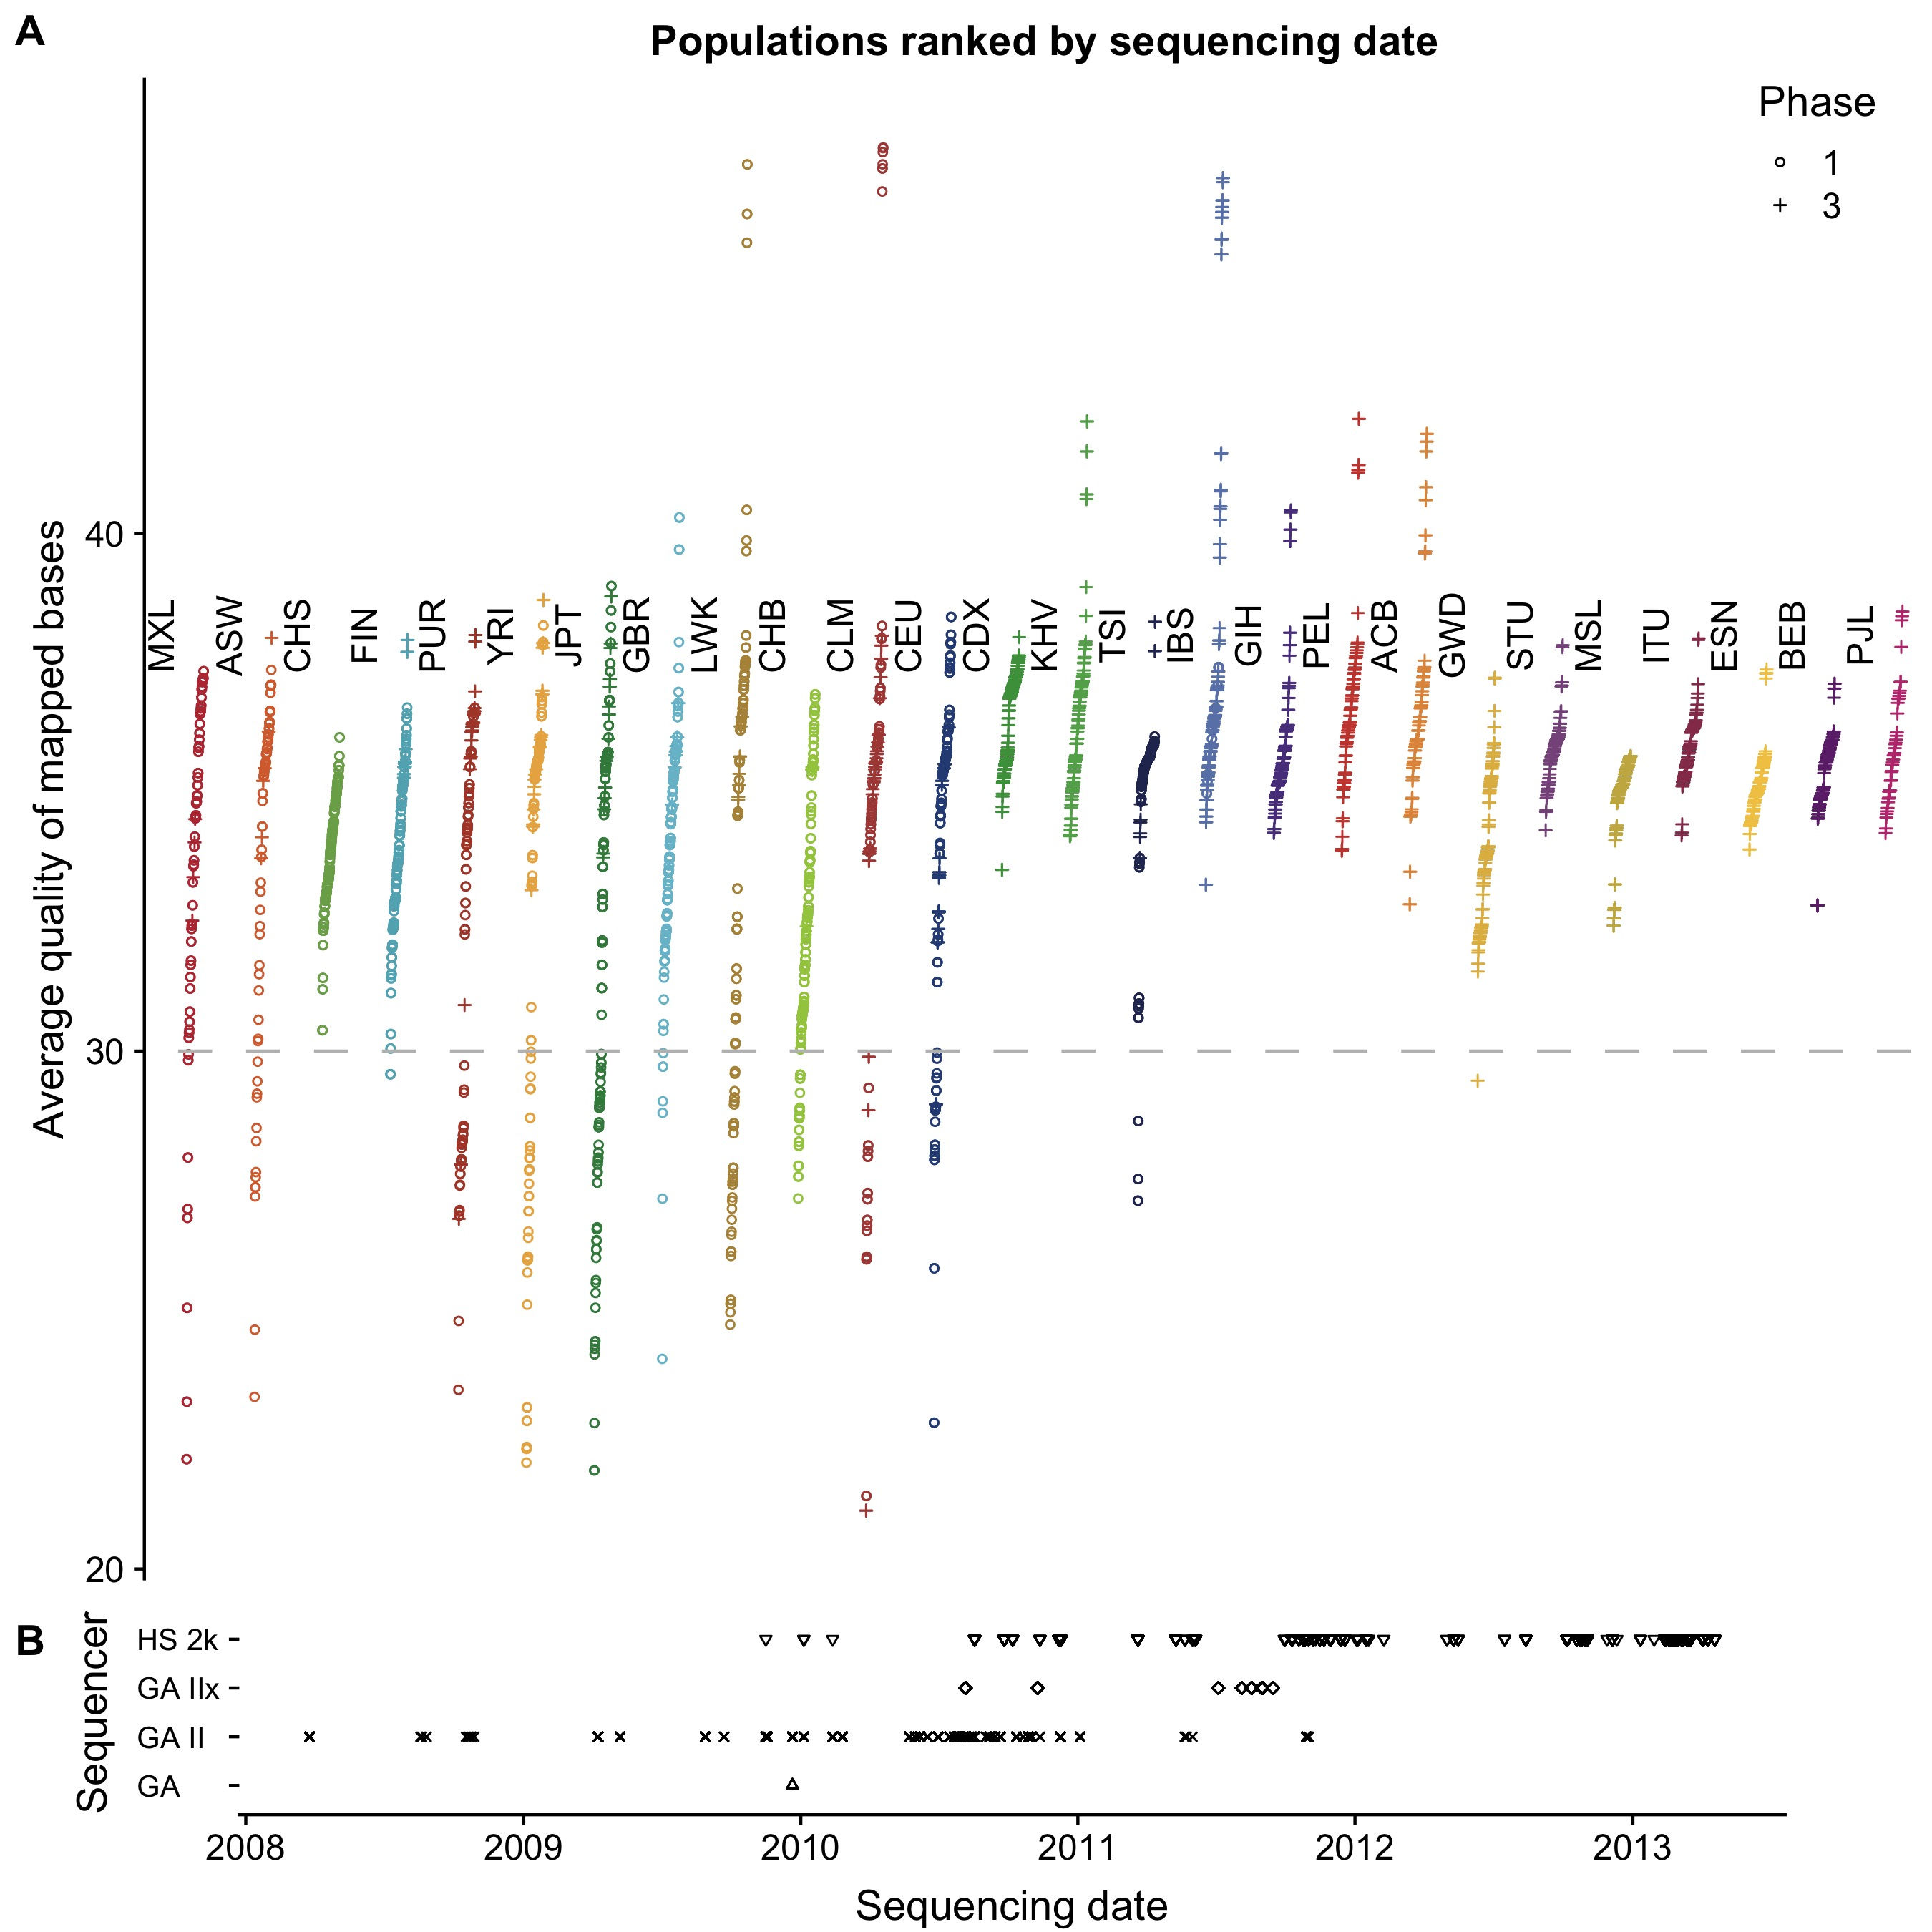
\includegraphics[width=\hsize,keepaspectratio]{./Figures/MapQualOverTime.jpg}

\caption{\textbf{A}The average quality of mapped bases for each individual per population included in the 1000 Genomes sequencing project. Individuals are ranked by the date of the earliest sequencing data is used for individuals sequenced more than once. The x-axis is ranked by the mean sequencing date per population. \textbf{B} The x-axis is sorted by the sequencing date per individual. The colours indicate the sequencing centres that produced the data for each individual and the shape indicates whether the individual belongs to Phase 1 or Phase 3 of the 1000 Genomes project. The bottom plot indicates the sequencing technologies used over time.}
\label{MapQual}
\end{figure}

\subsection{Overlap of significant SNPs}
The reverse GWAS approach similarly identified mapping-quality--associated SNPs in 24 of the 26 populations in the 1kGP.
Over 3517 variants were independently associated to low quality in at least two populations  (Figure \ref{OverLap}), and 3990 SNPs were significant after a meta-analysis (taking the sum of the deviations from each population and adjusting the degrees of freedom for the chi-squared test according to the number of populations with a segregating variant), as shown on Figure \ref{Manhattan}.  
\sgcomment{Look at the frequency distributions of these SNPs in GnomAD}

\begin{figure*}
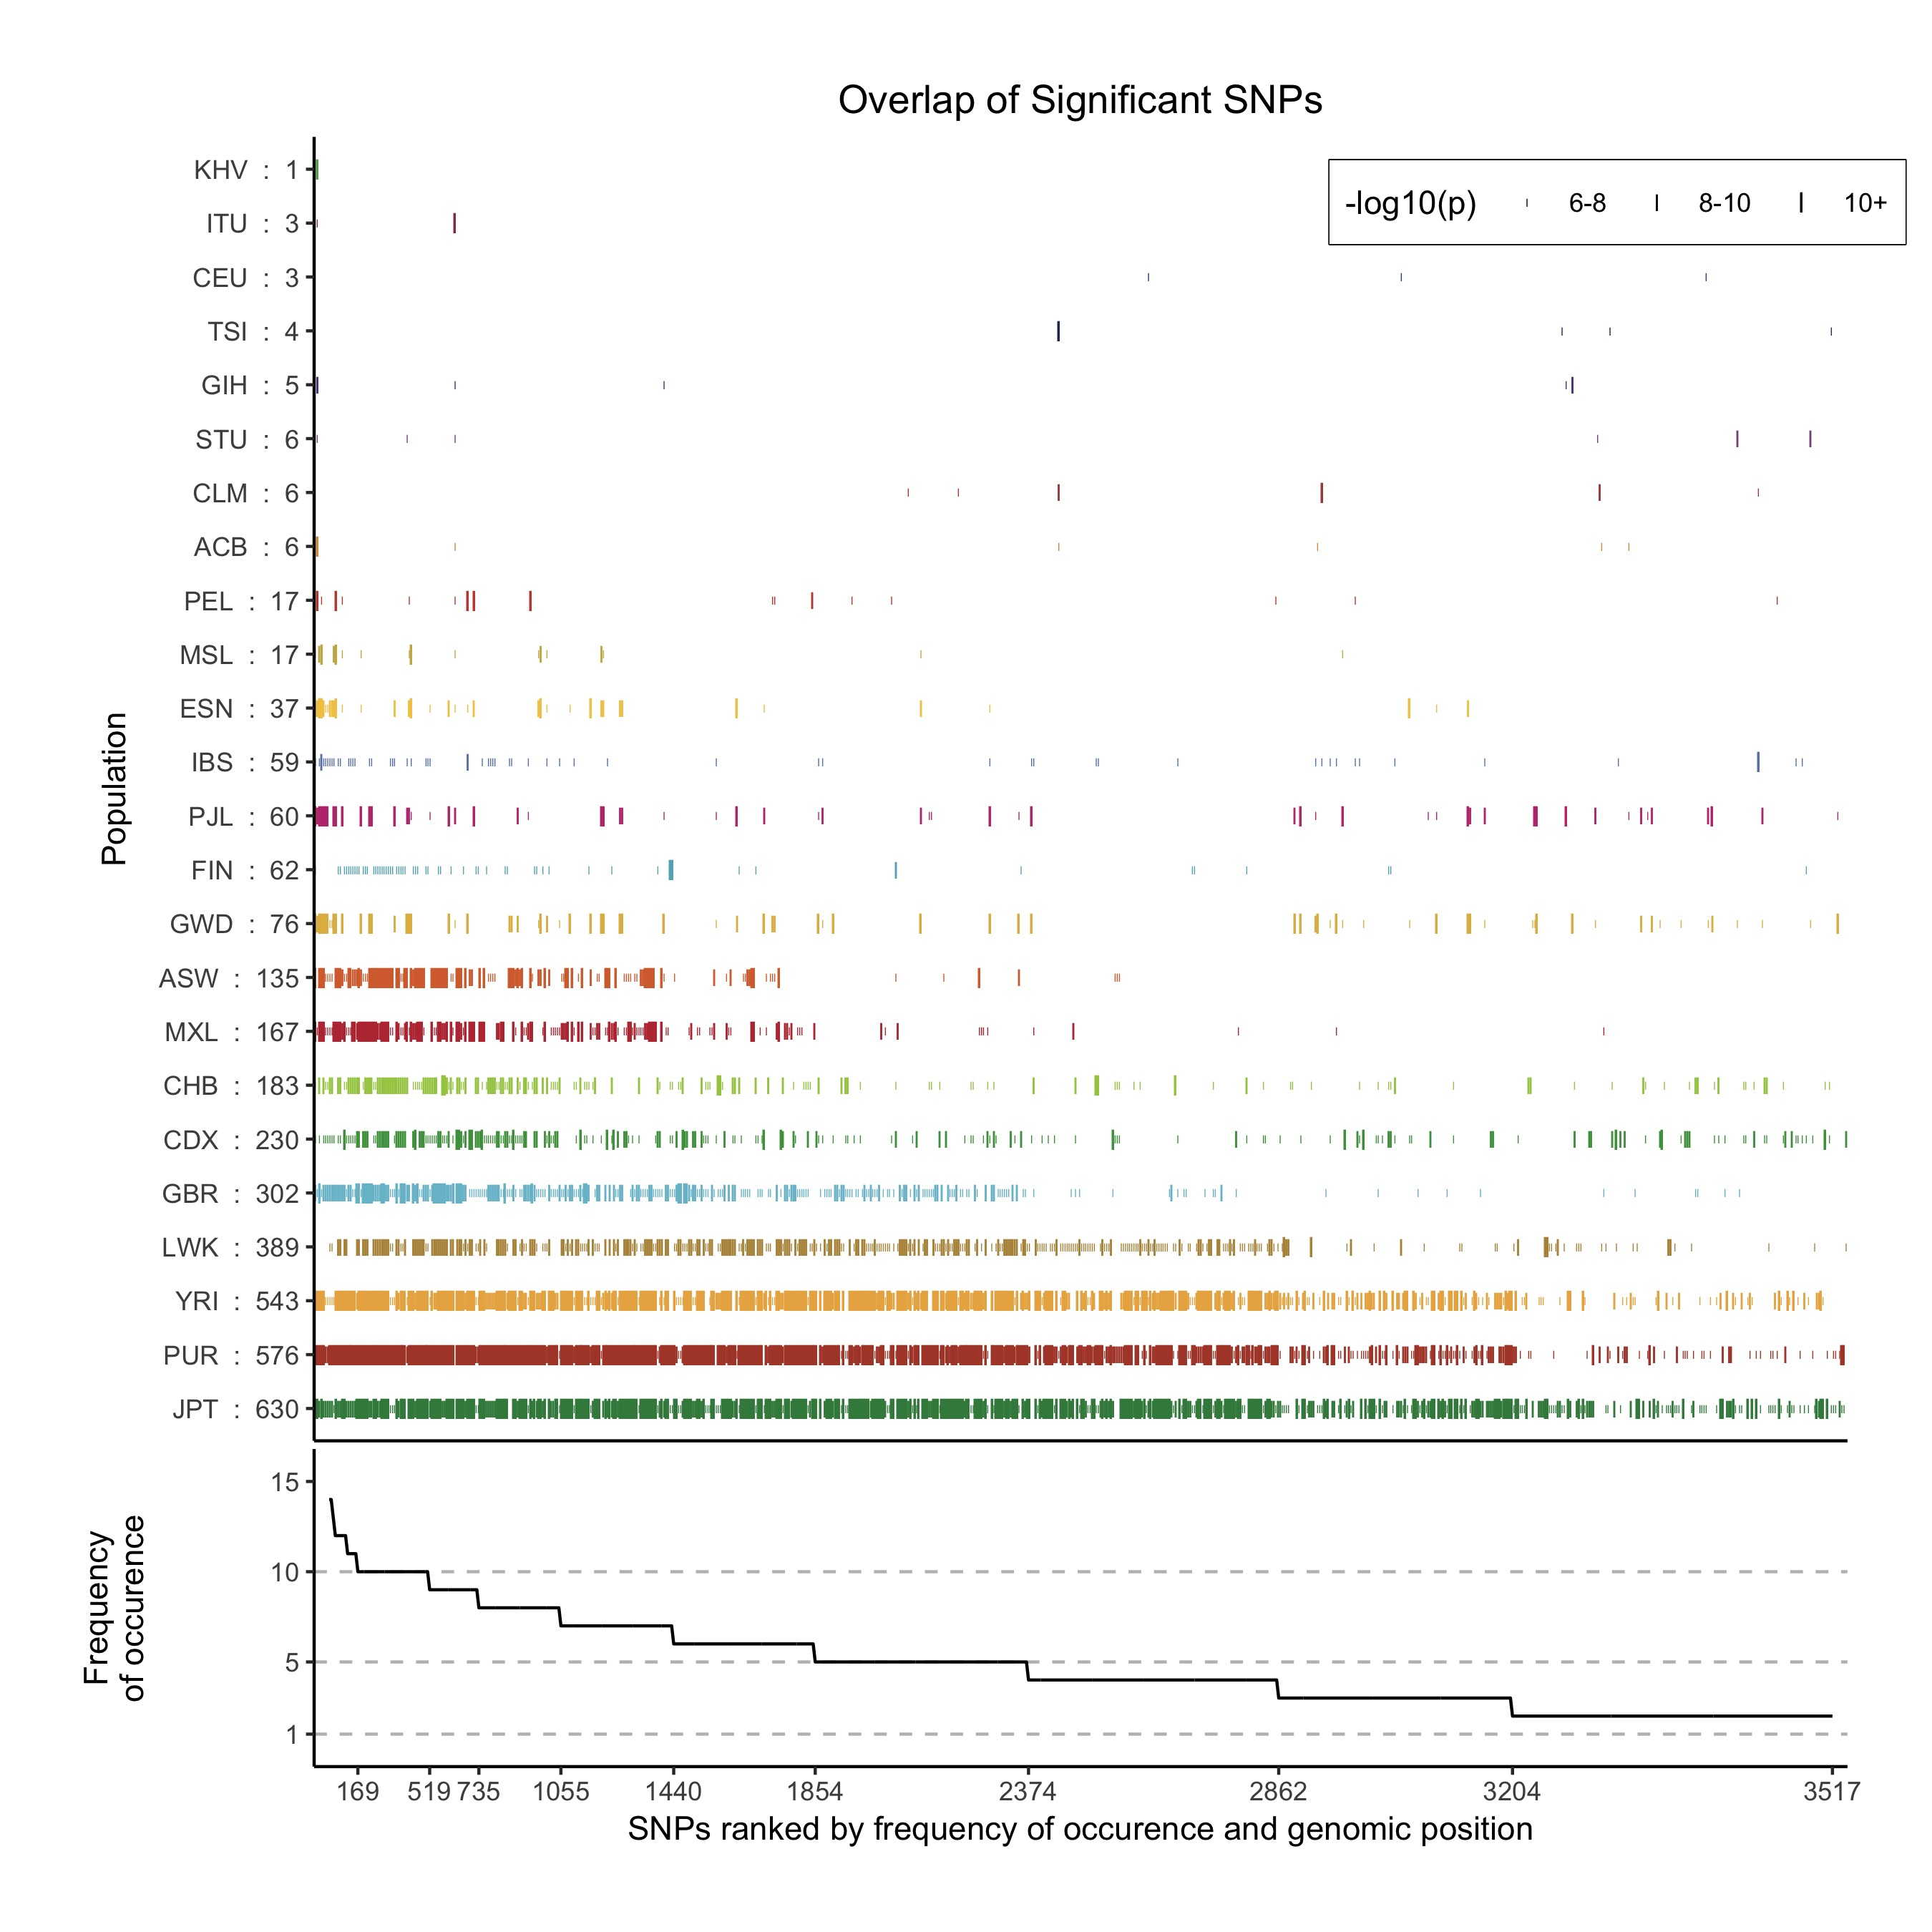
\includegraphics[width=\hsize,keepaspectratio]{./Figures/SNPOverlap6.jpg}

\caption{Overlap of SNPs identified independently to be associated with quality. 
The size of the crosses ( + ) are proportional to the -log10(p) value of that SNP.
The x axis is ranked by the frequency of occurrence of a SNP, then by genomic position.
The line plot underneath shows the number of populations for which a variant has reached significance.
The populations that tend to have the most low-quality individuals also tend to have the most variants associated to quality. 
The same variants identified as being low quality independently in each population are found in other populations. }
  \label{OverLap}
\end{figure*}

\subsection{Imputation}
The state of the art imputation servers use a combination of many databases including many that are not freely available.
From the perspective of researchers, they act as black-box imputation machines that take observed genotypes as input and return imputed genotypes.  
In order to investigate the proportion of variants that we've identified as being associated to quality that are being imputed, we submitted genotype data from all of the 1kGP individuals to the Michigan Imputation Server, and found that all of the SNPs we identified as being associated with quality for chromosomes 1 and 2 were imputed. This suggests that the imputation reference panel likely includes individuals with low sequence quality, and the dubious variants have not been removed. 
%\sgcomment{All of them? How is it possible if we only submitted Japanese? Also, I thought that we had only submitted a couple of chromosomes.} 
%\luke{Submitted all of the 1kGP, queried the combined meta-analysis list of SNPs}
\sgcomment{It may be useful to impute some of the NAG data.} 


\subsection{Found to be included in other GWAS }
Once we identified SNPs that were clearly associated with low quality, we searched the literature for any GWAS that might have reported these dubious variants as being significantly correlated with some biological trait. 
The NHGRI-EBI Catalog of published genome-wide association studies identified two recent publications that had found variants to have either reached or nearly reached genome wide significance of $ p < 10^{-8}$.

One of these studies genotyped individuals and imputed the data using the HapMap II as a reference  database for imputation. \sgcomment{If they used HapMap, how did they get affected by the 1000 Genomes results?}
The other study used the 1kGP sequence data and cell lines directly.
Both papers used strict quality thresholds, including population genetic statistical tests such as the Hardy-Weinberg equilibrium test, deviations in expected allele frequency and sequencing data quality thresholds. 
They also removed rare alleles and alleles with high degrees of missingness. 
Despite using the state of the art quality controls, these erroneous variants managed not only to be imputed onto real genotype data, but they also reached genome wide significance for biological traits.

\section{Discussion}
			
\subsection{Twins Research Human Genetics}
\sgcomment{Had we ever discusssed that these GWAS hits were not genome-wide significant?}
This paper identified SNPs associated to ADHD using a GWAS on quantitative measures of ADHD symptoms.
While none of their SNPs reached significance below $ p < 10^{-8}$, they reported their results below significance below $ p < 10^{-5}$.
The data used was imputed genotype data using Hapmap II as the reference.
One of the top 25 SNPs in the GWAS on ADHD (rs6057648) was identified as being significantly associated to data quality.\cite{} 

While they are clear in reporting that these SNPs are not genome wide significant, one can imagine a meta-analysis using this dataset would include the false positive SNP we identified. 
Furthermore, the approach they used to impute genotype data for GWAS is very common.
%A literature search of the keywords 'GWAS Genotype Imputation' yielded 19,300 results. \sgcomment{What is this about??}

\subsection{PLos One}
This paper used the raw BAM files from the 1kGP to identify EBV copy number by comparing the coverage of mapped reads to EBV.
They did PCR confirmation of EBV copy number using 7 samples from some of the populations, however all of these samples have relatively high quality data.
They performed a GWAS on the EBV copy number and identified only one SNP with significance below $ p < 10^{-8}$. 
However they reported the SNPs reading significance below $ p < 10^{-6}$. 
Four of the SNPs in the top hits of the Asian populations (rs200655768, rs184202621, rs201255786, rs201761909) we're identified by our regression against data quality. \cite{} 

The EBV strain was used to transform B-cells from blood samples from the 1kGP into lymphobastoid cell lines.
This is a commonly used transformation that helps preserve cell lines for long periods of time.
It's unclear what exactly might be causing the association to EBV copy number and the data quality, however, one could speculate that perhaps different protocols were used in the cell culturing of certain samples from the 1kGP which might affect the replication of the virus in the cells, or somehow affect the overall quality of the sequencing data produced.
Further investigations in the source of the issue could be done using the raw sequence data from the 1kGP along with the per sample per base quality metrics. 			

\subsection{Technical Artifact}
\sgcomment{needs some editing}
The variants identified in this study are likely to be technical artifacts from legacy technology.
If these sequencing platforms are no longer being used then it it likely that these artifacts are no longer being actively introduced in recent sequence data.
However, because the 1kGP data is widely used as a reference database, these variants are being imputed onto new genotype data.
We have shown that these variants have been significantly associated using traditional GWAS methods.
However this is not the only method that would be affected by these false positives. 
Polygenic risk scores, meta analyses and other methods that combine the scores of multiple variants might also include some of these variants in their analyses.
The inclusion of these variants could also affect population genetics analyses that compare and contrast populations based on allele frequencies.
luke{Multiple explanations for the signal, technical artifact, cell line artifact. The presence of these SNPs in the HapMap suggests a cell line effect, however with only 1\% of sites identified in 1kGP present in HapMap it's not a smoking gun.}

\subsection{Recommendations}
\sgcomment{needs some editing}
The most conservative approach would be to remove all individuals that don't meet the quality threshold as well as all the variants associated to low quality.
In this case, we used a cut off of an average quality of mapped bases over 30. 
It is the minimum requirements for \todo{GATK variant calling} for them to have a minimum quality of 30.
Another approach is to remove all the sites that reach a significance below $ p < 10^{-6}$ in at least two populations or using the sites reaching a significance below $ p < 10^{-6}$ in the combined test. (See supplementary material for lists of SNPs)
%\subsection{Power limits and Quality Controls}
%If these variants are truly spurious, why were they not identified by the Hardy-Weinberg test of heterozygosity?
%how many hetd do you need to detect HWE significance?
%We were able to identify many variants with frequencies below \todo{the power threshold for HWE}.

%\subsection{Technical Source of Error}
%B tail trimming  (Minoche et al. Genome Biology 2011)
%issues with PCR?
%repetitive regions, GC bias...

\section{Conclusion}

On a technical front, we were surprised that strong correlations between SNPs and technical covariates in the 1kGP project had not been identified before. The reverse GWAS approach is rather straightforward, and should probably be a standard in a variety of -omics studies. 

More generally, to improve the quality of genomic reference datasets, we can proceed by addition of new and better data and by better curation of existing data. Given rapid technological progress, the focus of genomic research is naturally on the data generation side. However, cleaning up is also important to avoid generating spurious results. The present findings suggest that a substantial fraction of the final release of the 1kGP project is overdue for removal or re-sequencing. 

Somewhat embarrassingly, we have not identified the precise mechanism through which the technical artifact was introduced: we have ruled out neither cell-line, sequencer, nor algorithmic artifact. Given that modern platforms seem to have resolved this technical issue but that recent studies continue being affected by the legacy batch effect, we found it worthwhile to draw attention to the statistical artefact while the sequencing forensics investigation can take place.     


%but evidence points to the fact that the artifact disappeared in the later stages of the 1kGP, and does not corrupt more recent data.   
 
%As more large scale genotyping efforts are being imputed on the same legacy datasets, we must scrutinize the quality of the reference databases to avoid the propagation of false positives. 
%These results bring forth many questions regarding the reliability of legacy datasets. 
%Moreover, since there are so many broad applications of imputation, it frames the question for reference data turnover. 


%Our method identifies spurious mutations by correlating mutations with data quality metrics. 
%We propose including our quality control methods to identify possible false positives in sequencing data. 
%We have focused on the 1000 Genomes Project dataset as its quality metrics were freely available, however the issues of quality control are not limited to this one consortium. 
%This study only used one dataset and one quality metric, but using this same approach can be used to identify more false positives in many more datasets. 


%Many types of DNA sequencing machines have been available on the market over the past decade.
%Different types of sequencing technologies can have different technical limitations in quality control.
%This makes combining data an issue especially when multiple sequencing technologies are involved in the data production.
%Many of the legacy datasets produced using dated sequencing technologies have been known to contain a higher rate of false positives than their more recent counterparts.
%The errors in one dataset do not disappear when they are combined with another higher quality one.
%The technical biases caused by legacy sequencing technology is becoming increasingly relevant as newer technologies produce data with lower error rates, and more stringent quality controls.




\section{Methods}
\subsection{Metadata}
The metadata used in this analysis was compiled from each of the index files from the 1000 Genomes file system. 
Average quality of mapped bases per sample was obtained from the BAS files associated with each alignment file. 
Each BAS file has metadata regarding each sequencing event for each sample. 
If a sample was sequenced more than once, we took the average of the each quality score from each sequencing instance. 
The submission dates and sequencing centres for each sample in the analysis was available in the sequence index files.  
This file also has multiple entries per sample, however, we were unable to match the individual sequencing runs between the bas files and the index file, which lead us to take the average of the quality scores and only kept the earliest sequencing date per sample. 
The dates of the sequencing are only used to plot Figure.

\subsection{Data Availability}

Index of BAS files \href{http://ftp.1000genomes.ebi.ac.uk/vol1/ftp/data_collections/1000_genomes_project/1000genomes.low_coverage.GRCh38DH.alignment.index}{available here}.

Phase3 analysis sequence index file  \href{http://ftp.1000genomes.ebi.ac.uk/vol1/ftp/phase3/20130502.phase3.analysis.sequence.index}{available here} 

\todo{link to my compiled metadata file here}

\subsection{Quality Controls}
We reproduced the quality control pipelines used by Harris et. al as they applied the current state of the art quality thresholds to remove questionable sequences especially for the high standards for detecting population level differences. 
Several mask files were applied to remove regions of the genome that might be lower quality, or might have very different mutation rates or basepair complexity compared to the rest of the genome. 
The  1000 Genomes \href{http://ftp.1000genomes.ebi.ac.uk/vol1/ftp/release/20130502/supporting/accessible_genome_masks/20141020.strict_mask.whole_genome.bed}{strict mask} was used to remove low quality regions of the genome , highly conserved regions were removed using the \href{http://hgdownload.cse.ucsc.edu/goldenPath/hg19/database/phastConsElements100way.txt.gz}{phastCons100way} mask file and highly repetitive regions were also removed using the \href{http://hgdownload.cse.ucsc.edu/goldenpath/hg19/database/nestedRepeats.txt.gz}{NestedRepeats} mask file from RepeatMasker. 
Furthermore, only diallelic autosomal SNPs were considered, with missingness below 0.01, MAF less than 0.1, and MAF greater than 0.9.

\subsection{Genome Wide Association Study}
Using an in-house R script, we performed a logistic regression using the glm package. \cite{R,GLM} We performed this statistical test independently for each population of the 1kGP. The deviations from the null model for each test was used to compute the chi-squared p value for each SNP for each population. Since each deviation follows a chi-squared distribution, the sum of the deviations also follow a chi-squared distribution. However, since not all SNPs are present in all populations, when computing the p values for the summed deviations, the degrees of freedom were adjusted to the number of populations tested. 

\subsection{Mutation Spectrum}
We calculated the mutation spectrum of triplets for the list of significant SNPs for the JPT population using a similar method as described in Harris et al. 2017. \cite{Harris2017a}
We modified the methods as necessary for our purposes, scripts are available \href{https://github.com/LukeAndersonTrocme/QualityPaper}{here}. 

\subsection{Imputation}
Using the Michigan Imputation Server, we imputed the genotype data from 1kGP for chromosomes 1 and 2.
We used the genotyped data from the 1kGP \href{ftp://ftp.1000genomes.ebi.ac.uk/vol1/ftp/release/20130502/supporting/hd_genotype_chip/ALL.chip.omni_broad_sanger_combined.20140818.snps.genotypes.vcf.gz}{Omni chip} genotype data.
The VCF file returned from the server was then downloaded and used to search for the number of significant SNPs successfully imputed.

\section{Code Availability}
https://github.com/LukeAndersonTrocme/QualityPaper

\section{Acknowledgments}
We would like to thank Kelly Harris for sharing her mutation spectrum scripts.


%\bibliographystyle{plain}
\bibliography{Legacy.bib}

\section{Supplementary Figures}
\renewcommand{\thefigure}{S\arabic{figure}}
\setcounter{figure}{0}   	

\begin{figure}
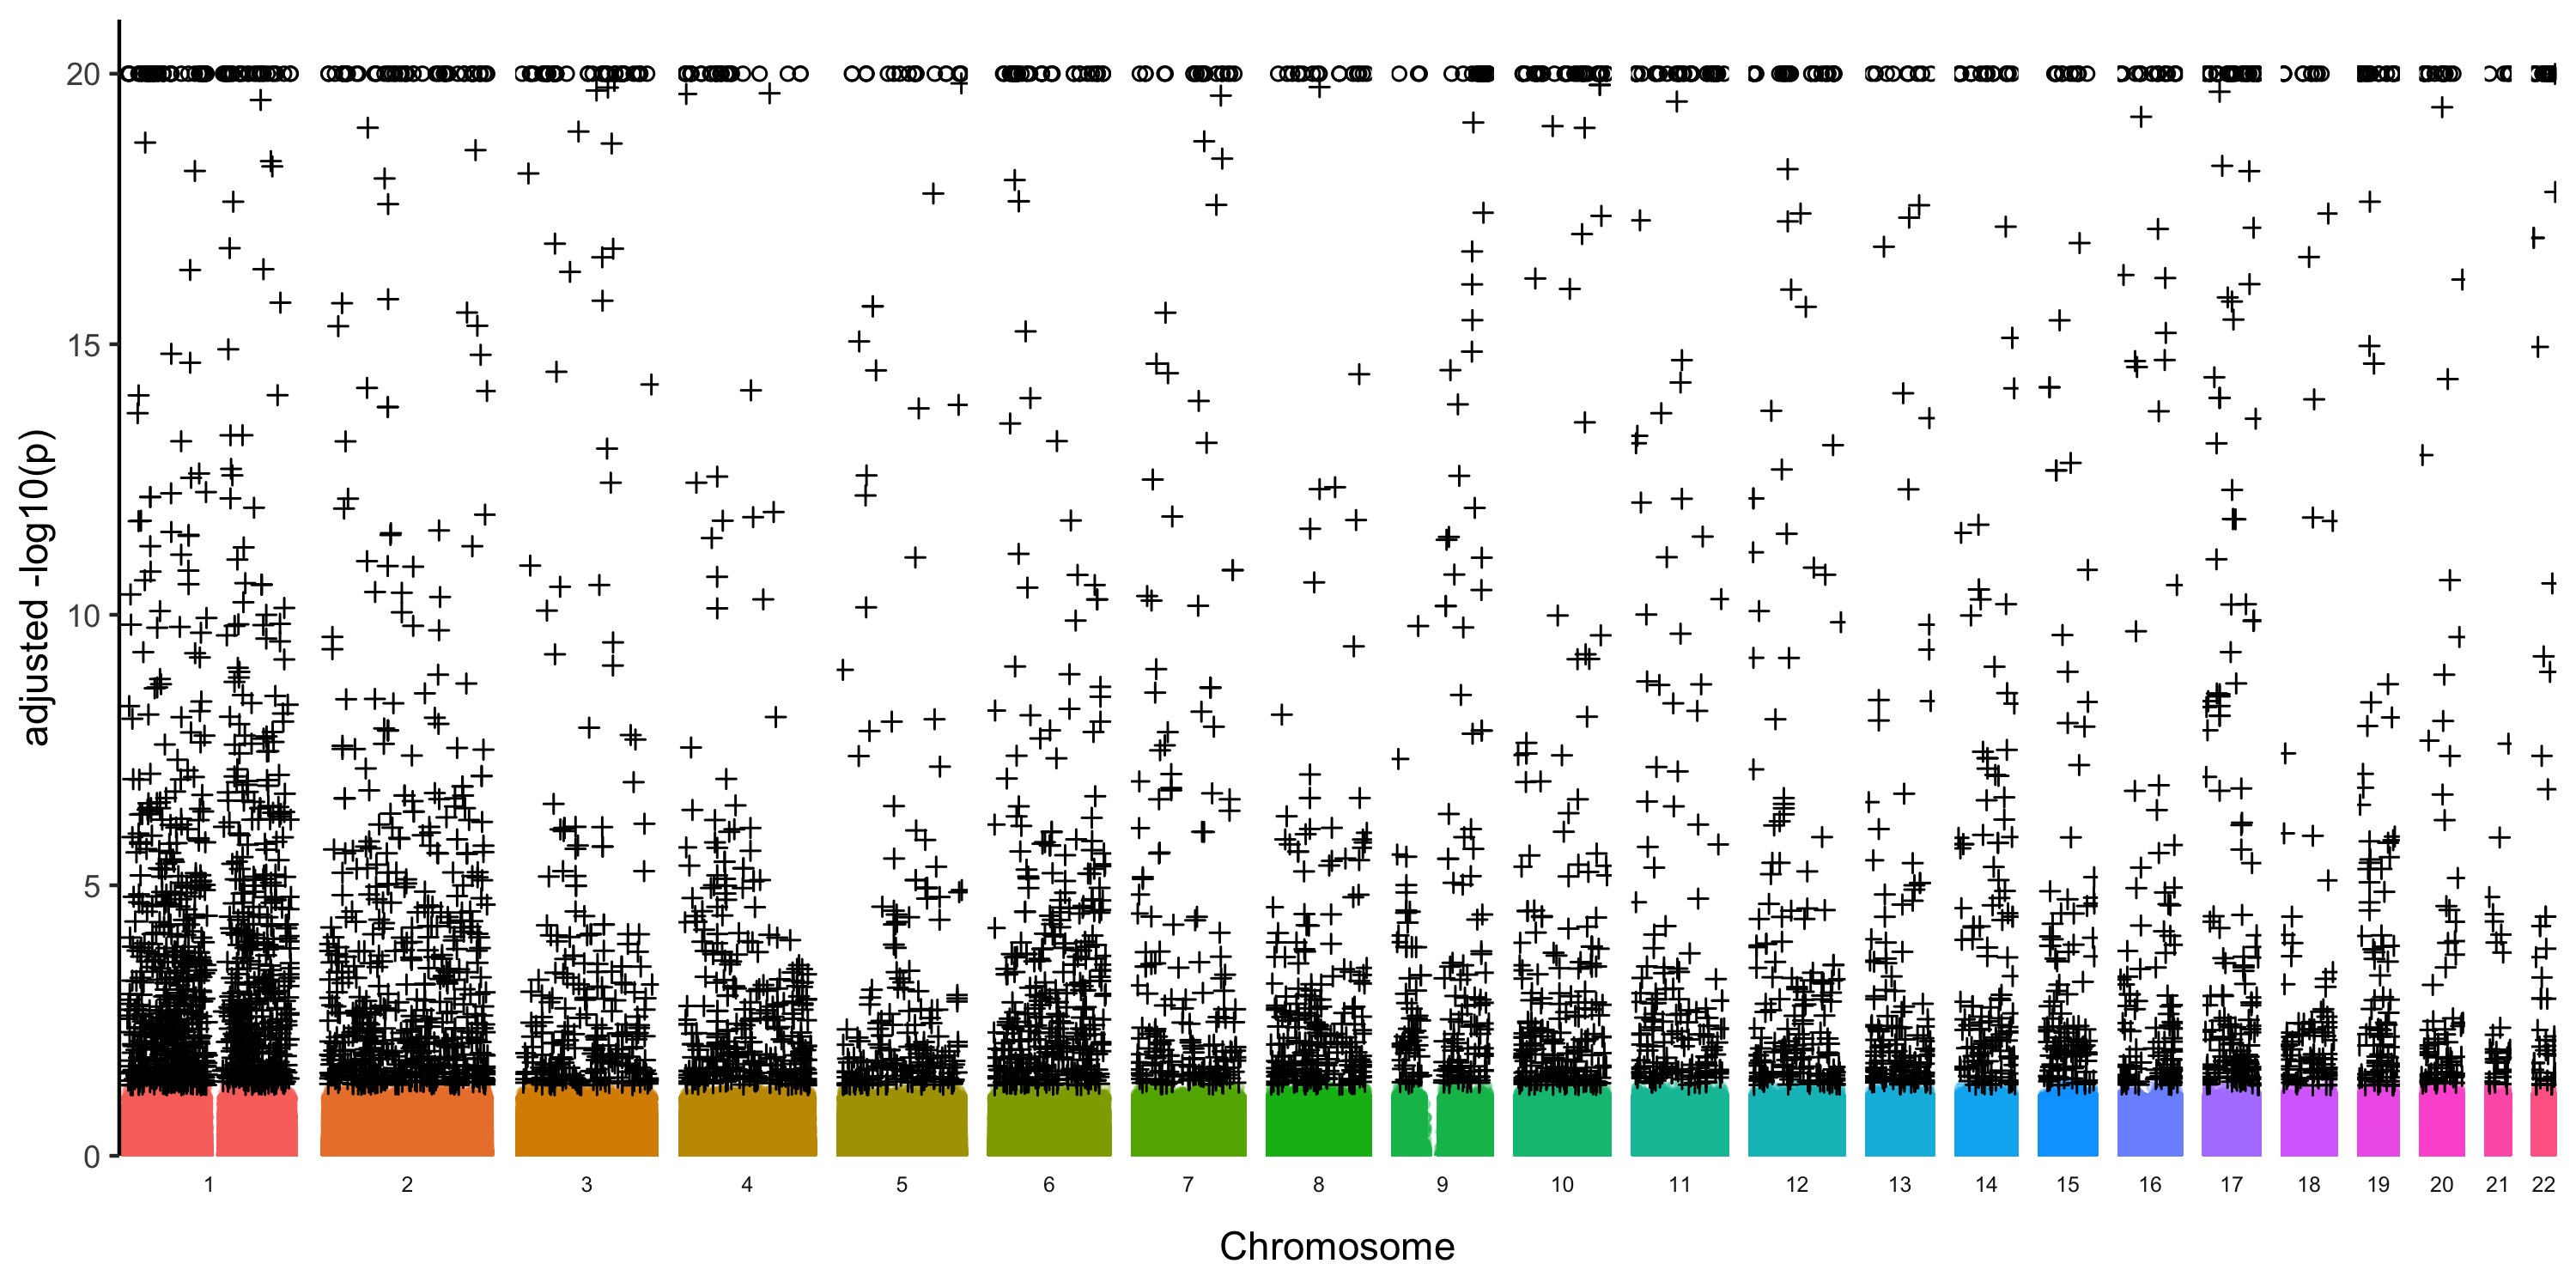
\includegraphics[width=\hsize,keepaspectratio]{./Figures/ManhattanPlot_adjusted.jpg}

\caption{Manhattan plot of the -log10 p values for the combined test using the deviations from each population of the 1kGP. 
There are 3990 variants that reach p values greater than $ p < 0.01$ after performing a two-stage Benjamini and Hochberg FDR adjustment. 
The circles ( o ) are SNPs that reached values greater than 20, for clarity we implemented hard ceiling at 20.}
  \label{Manhattan}
\end{figure}


\begin{figure}
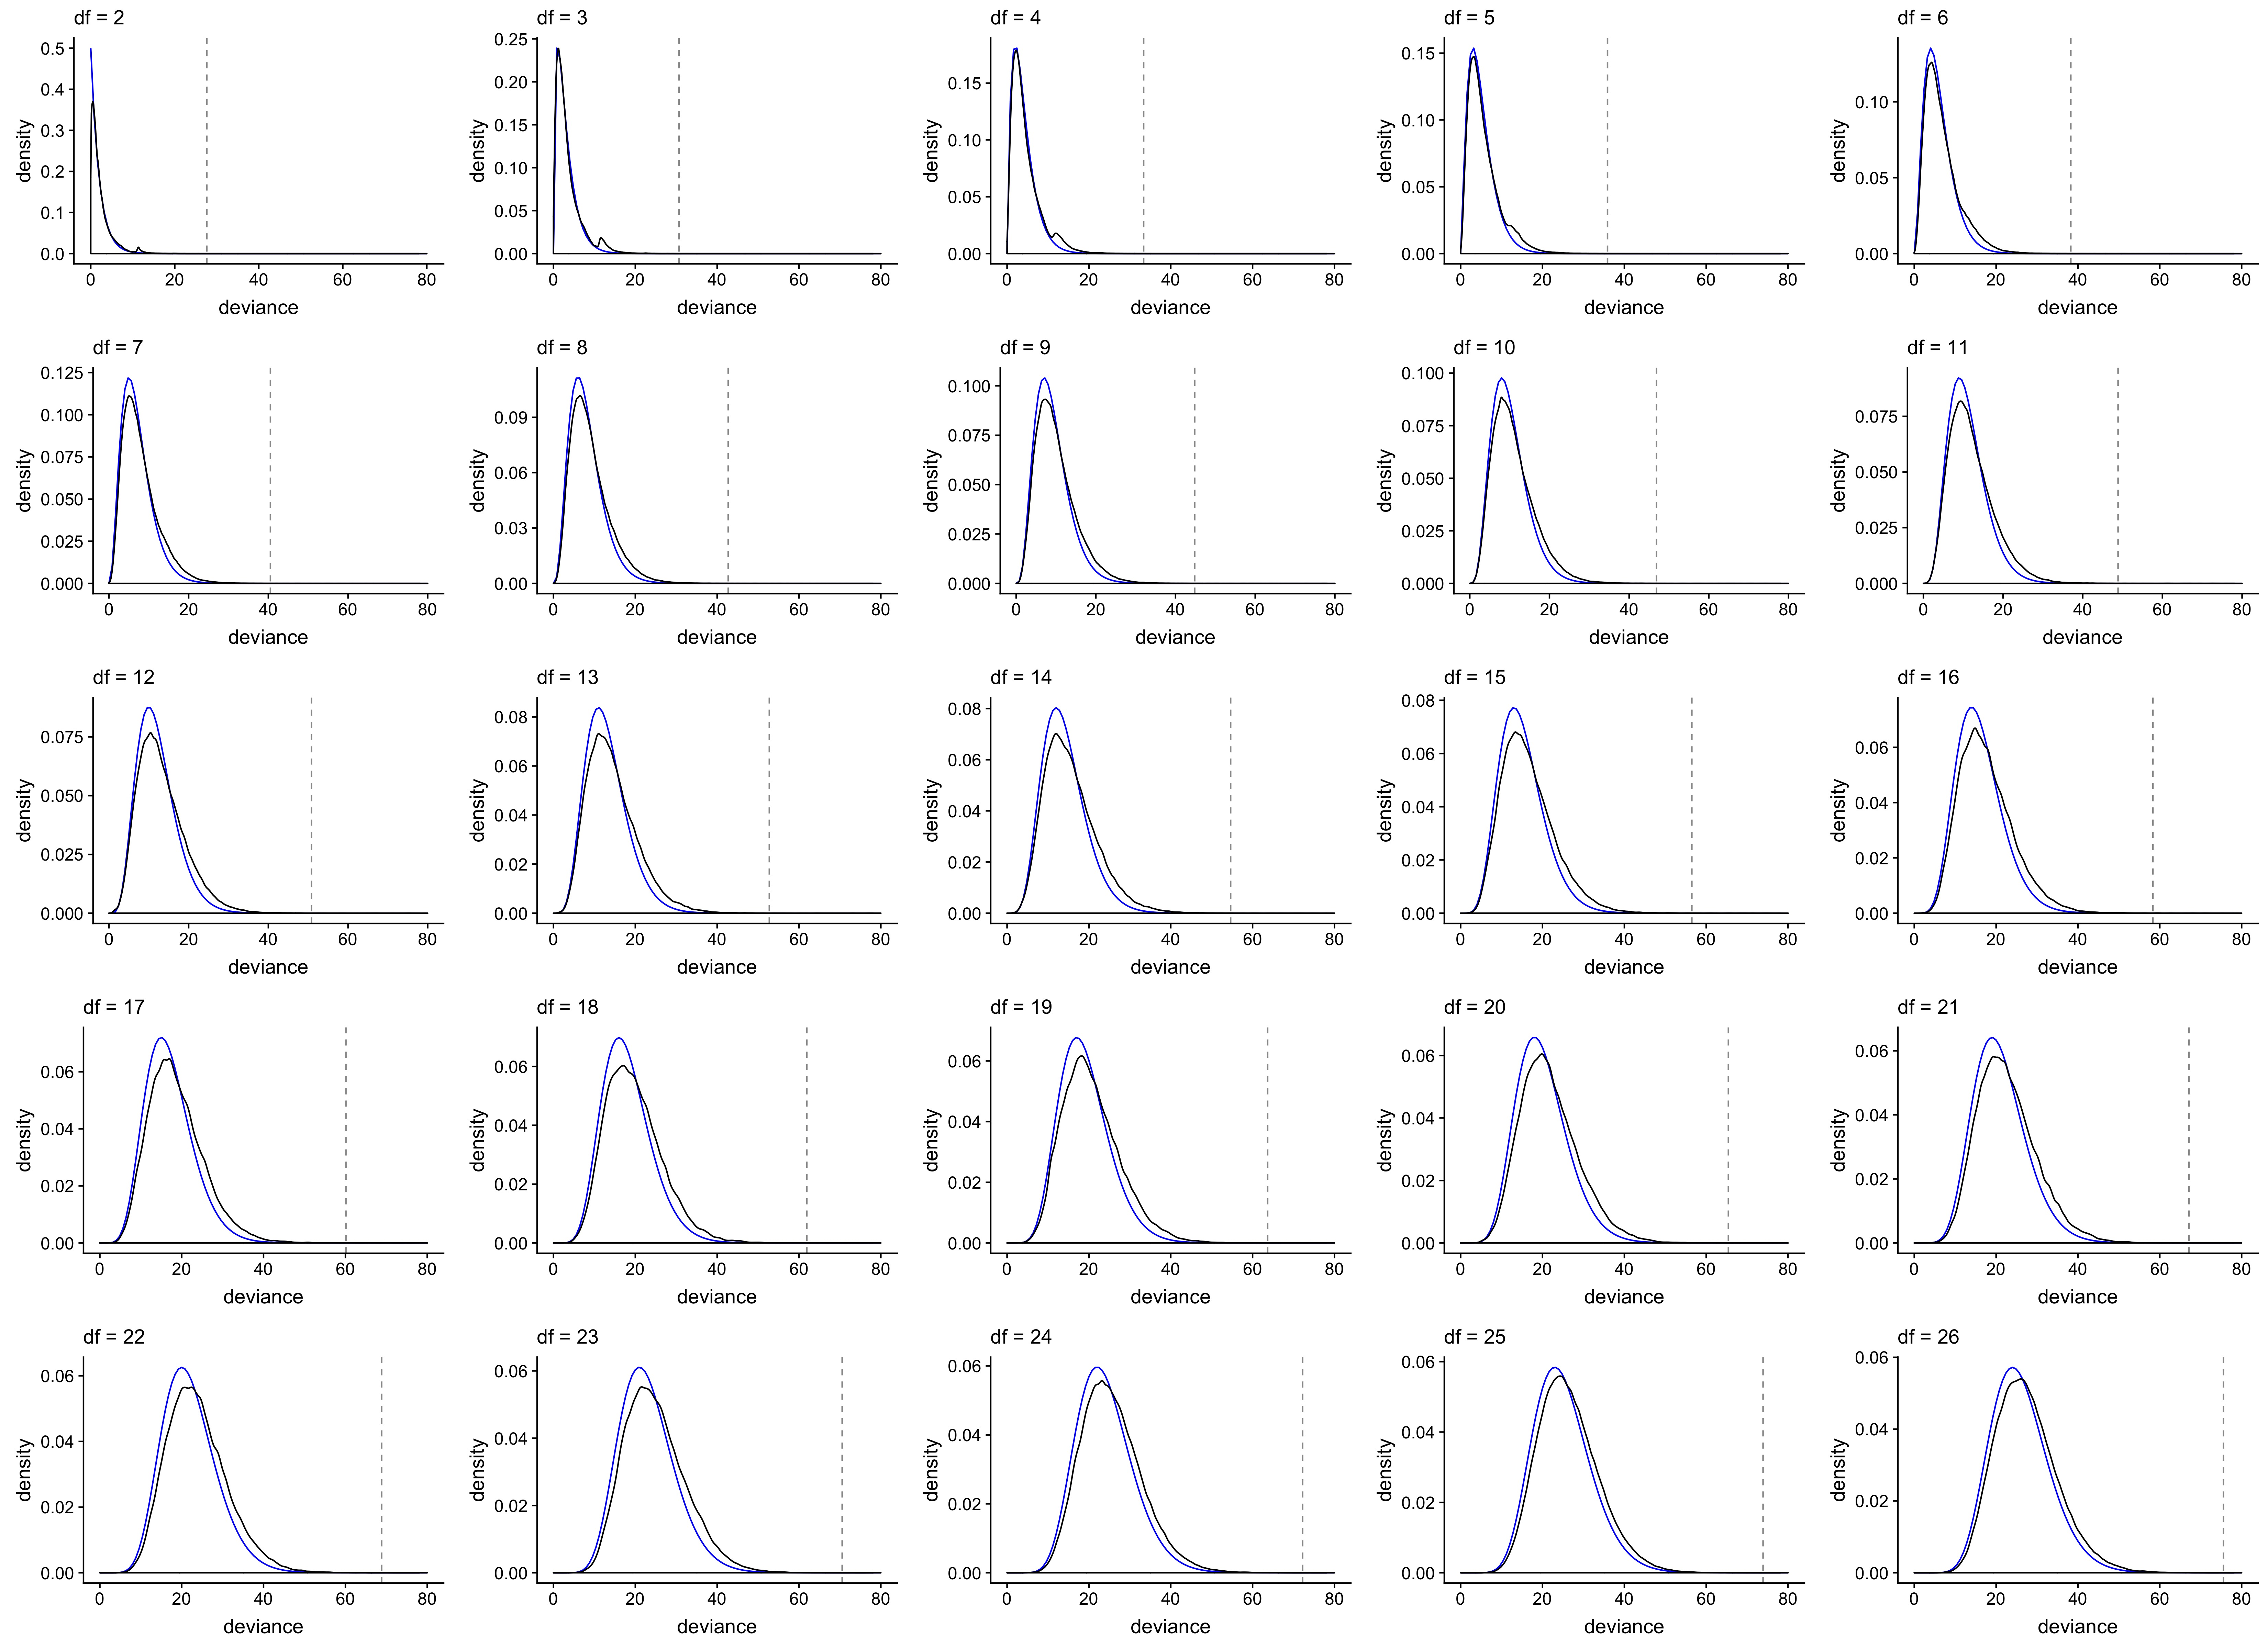
\includegraphics[width=\hsize,keepaspectratio]{./Figures/AllDeviances.jpg}

\caption{Empirical distribution plots of the sum of deviances grouped by N, the number of populations included. The blue curve is the theoretical null reference chi squared distribution with $N$ degrees of freedom. Note $\sum_i^N  \chi^2_1= \chi^2_N$. The grey dotted line indicated the significance level of $10^{-5}$ for the respective distribution which happens to be very close to the adjusted p value threshold at 0.01 FDR. }
  \label{Deviations}
\end{figure}

\begin{figure}
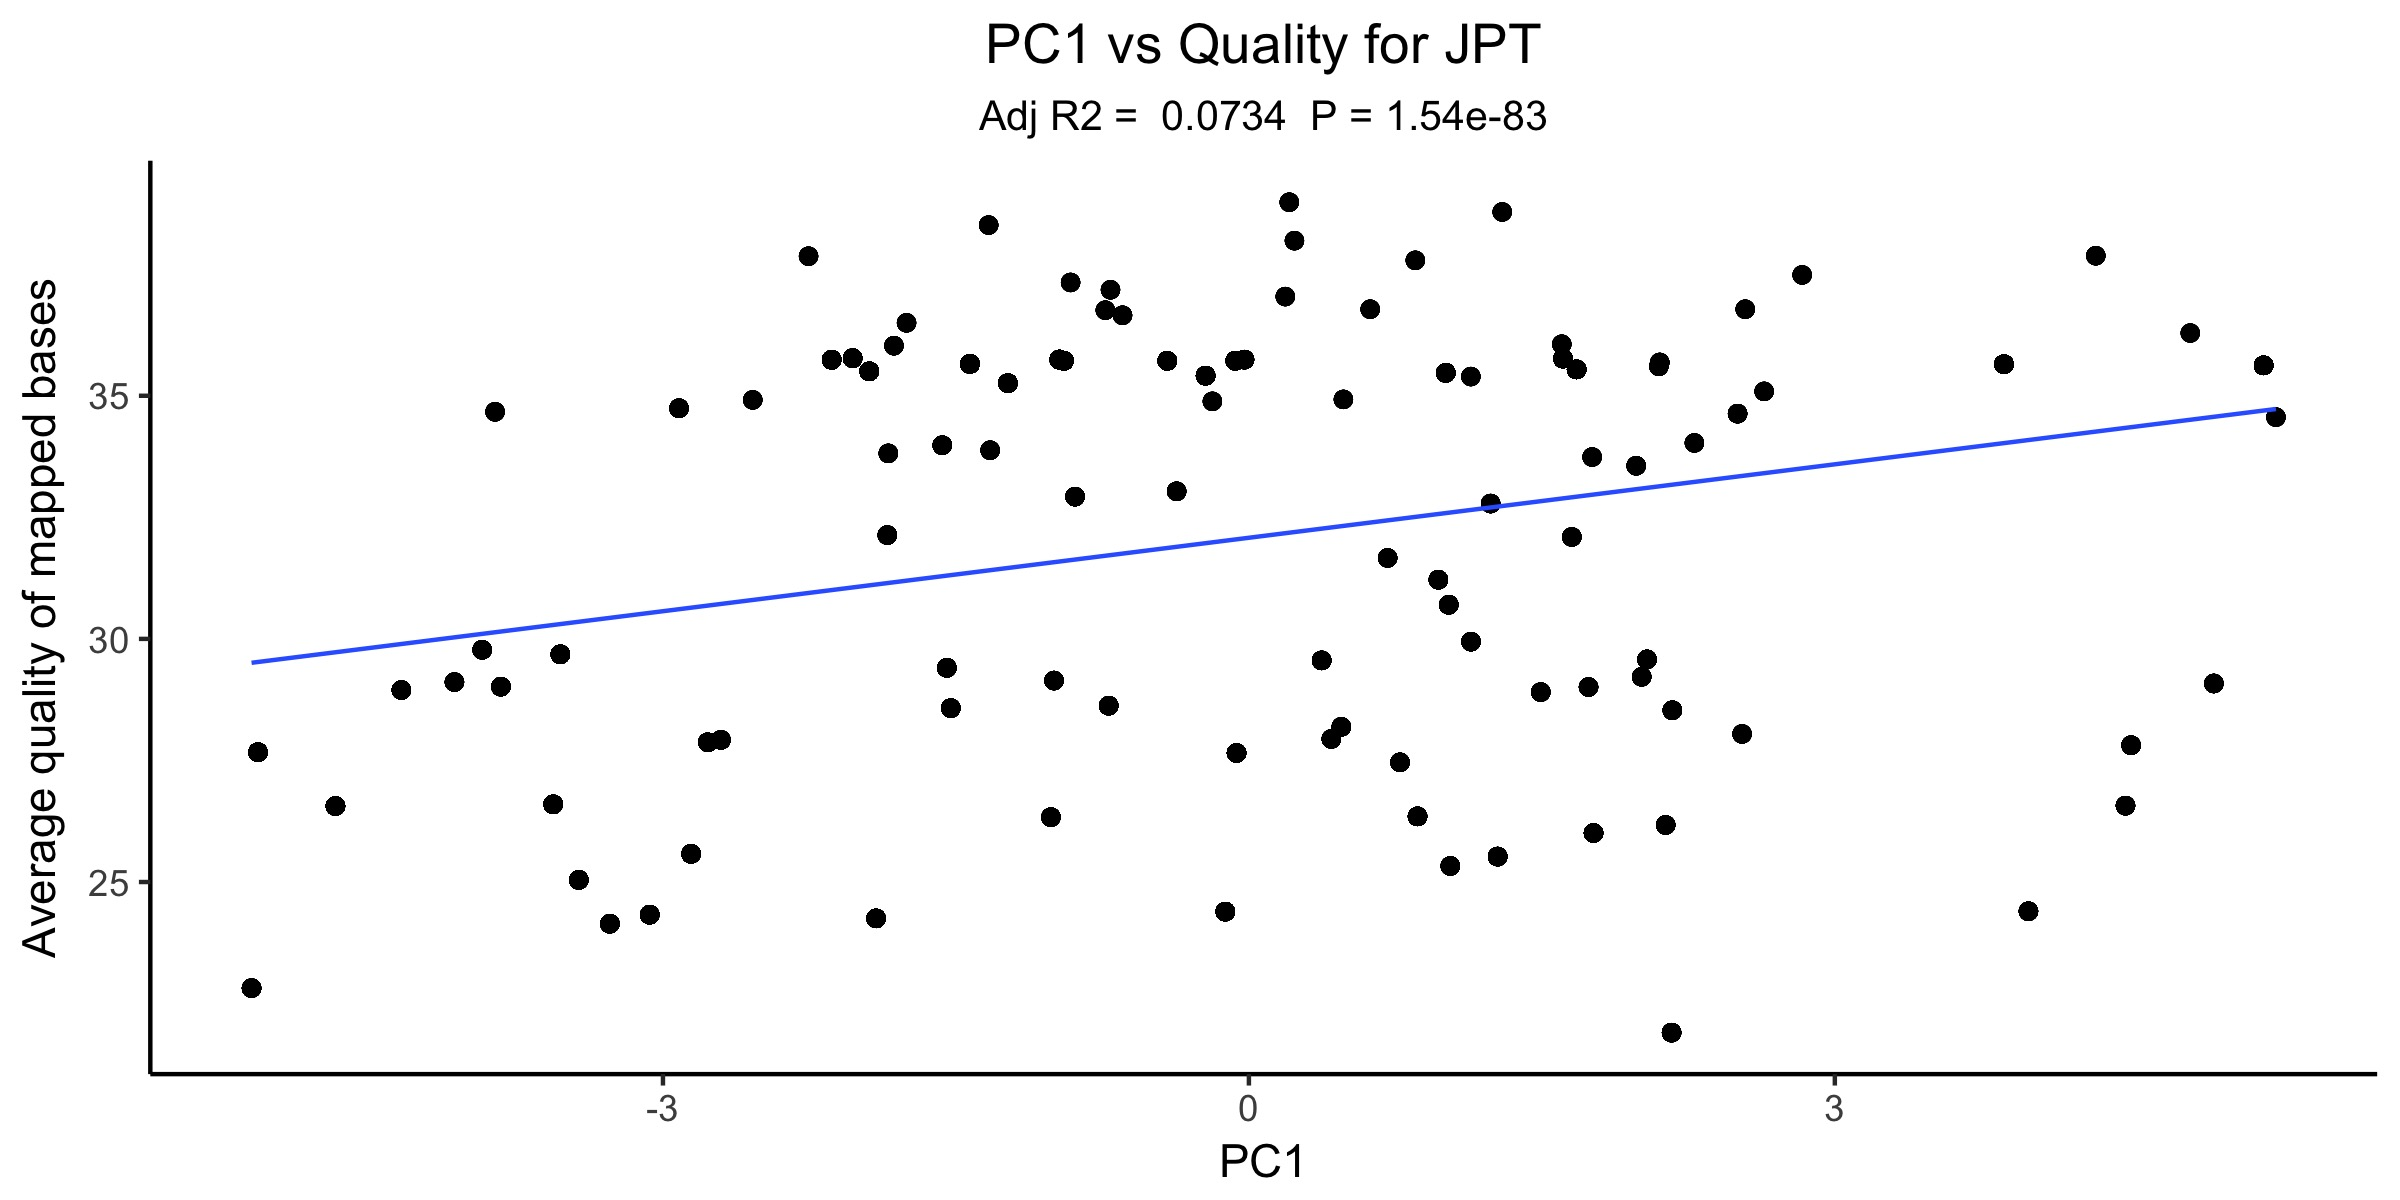
\includegraphics[width=\hsize,keepaspectratio]{./Figures/PC1_Correlation.jpg}
\caption{Regressions against mean quality per mapped base pair per individual is an excellent correlate with prevalence of the  *AC${\rightarrow}$*CC mutational signature in 1kGP, with individuals with low-quality data showing elevated rates of the signature.  }
\label{PC1_Correlation}
\end{figure}

\begin{figure}
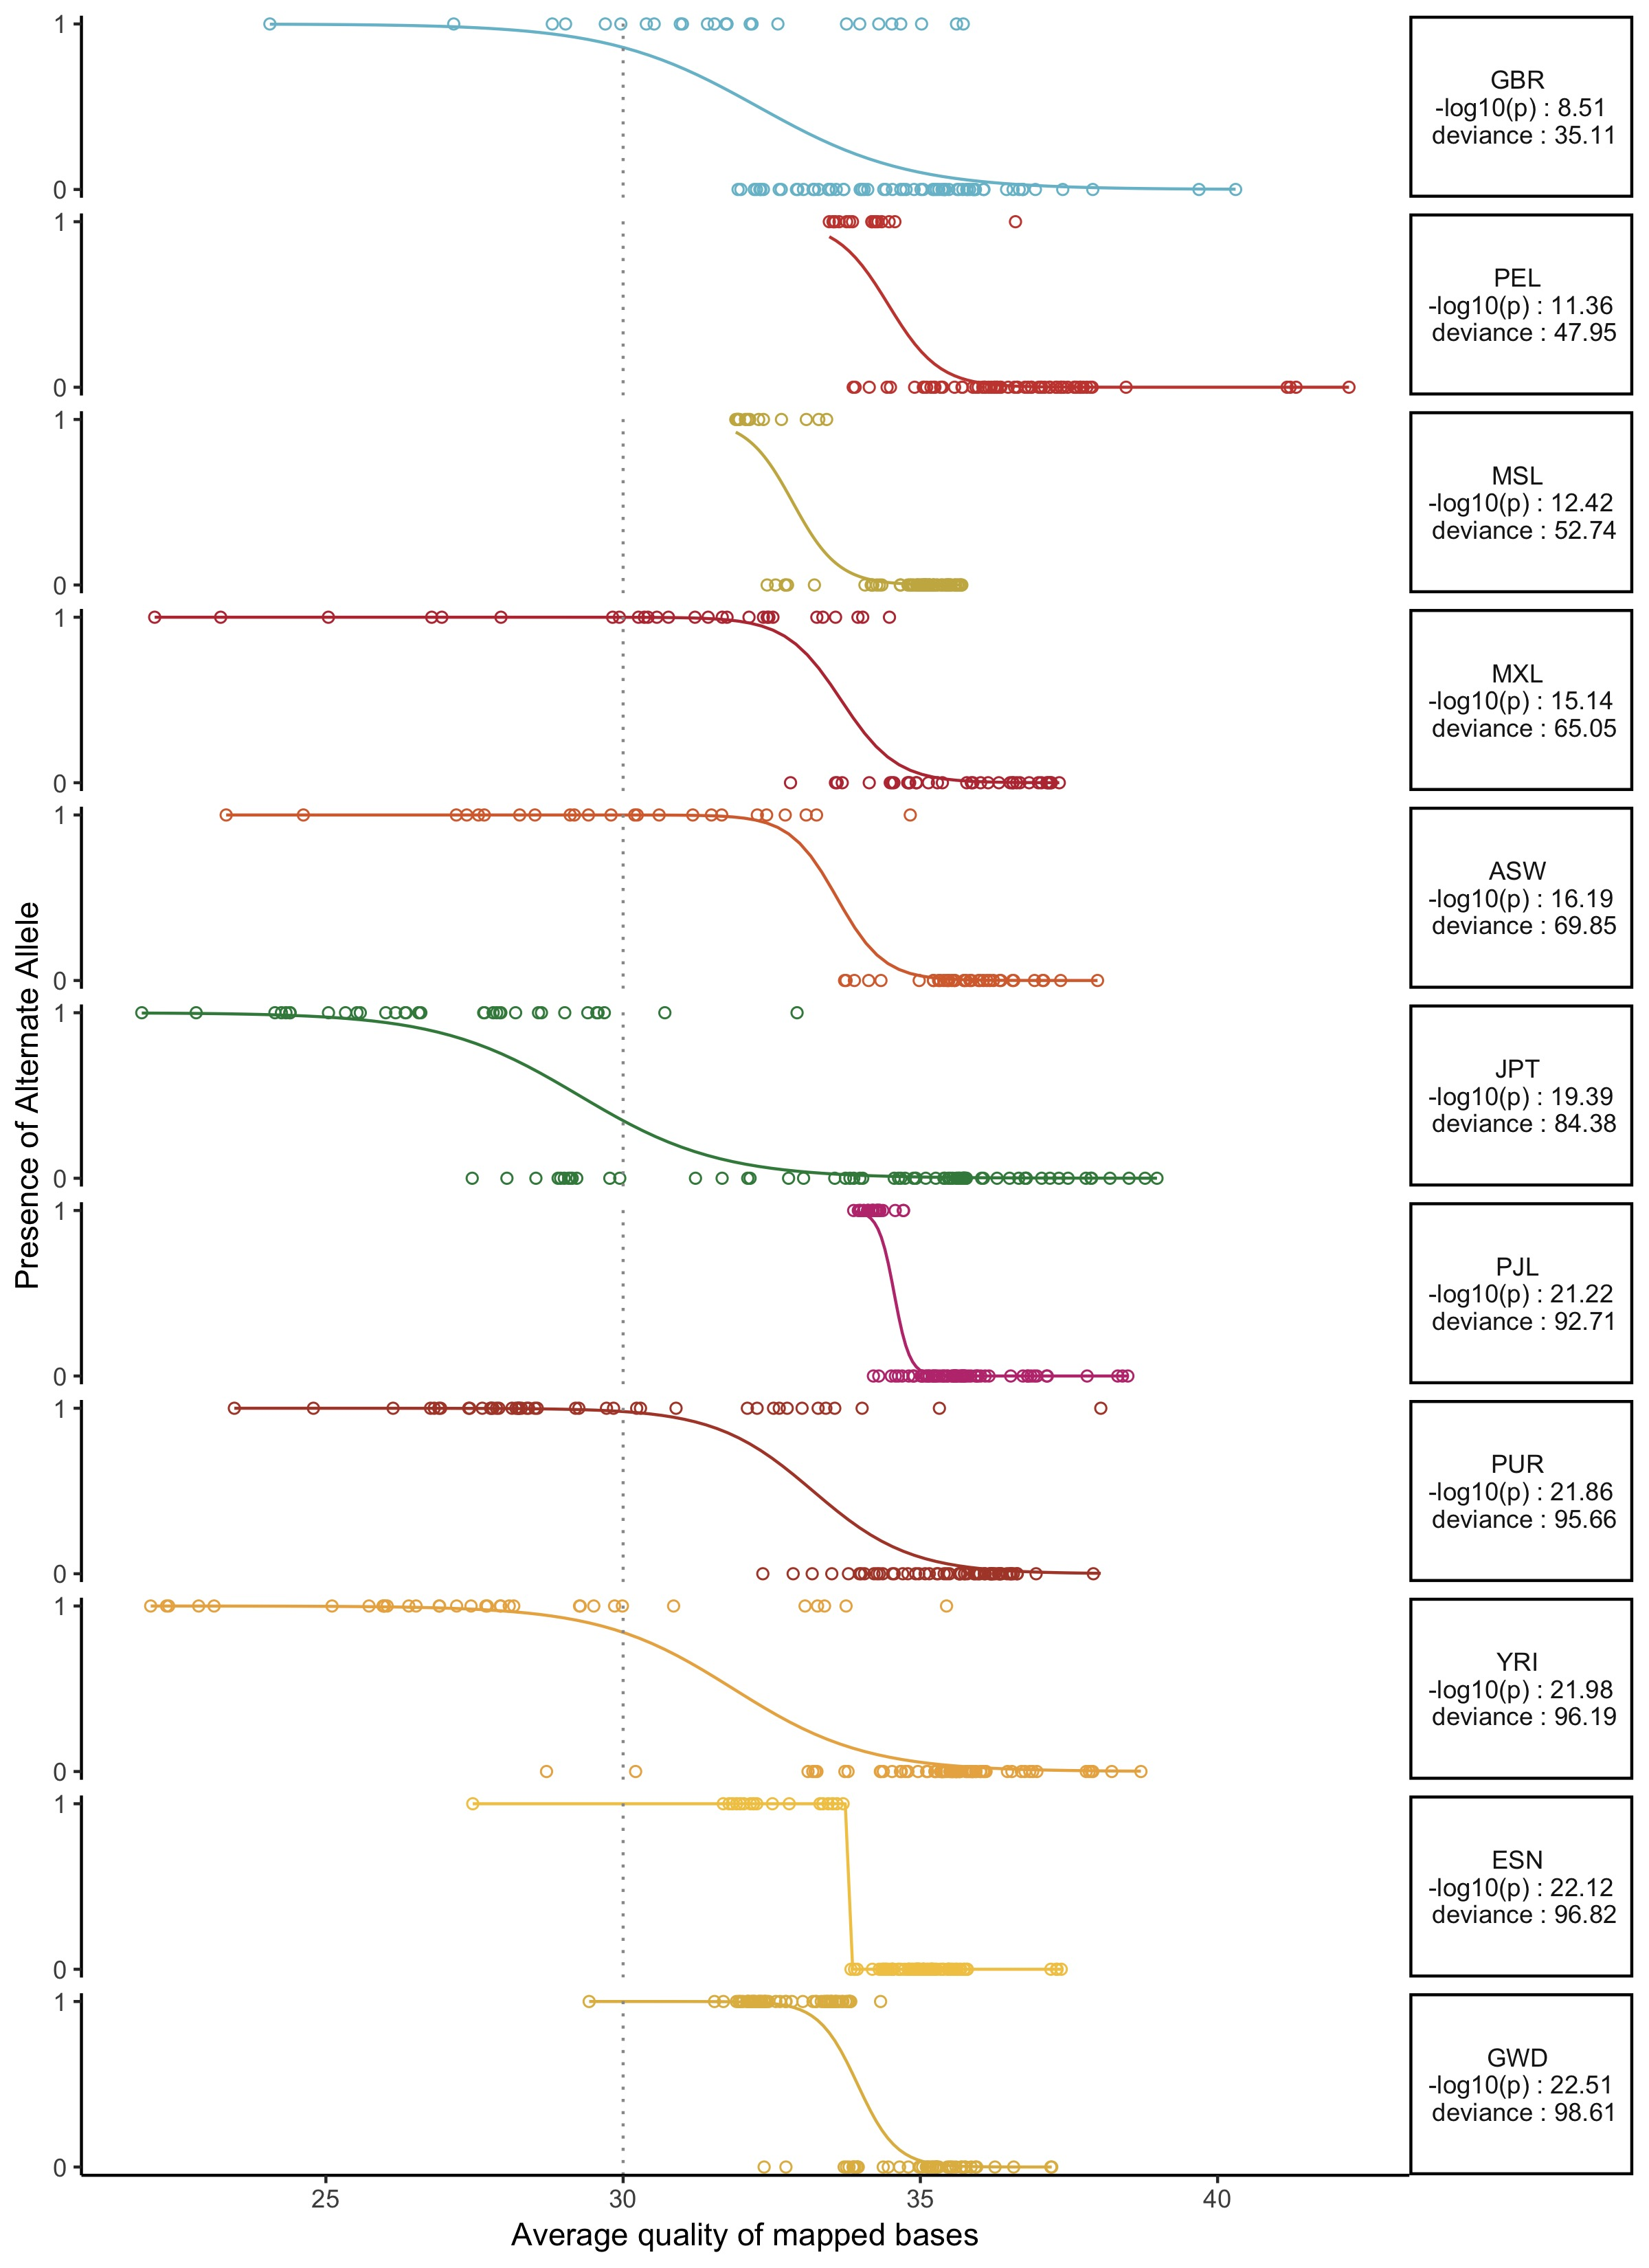
\includegraphics[width=\hsize,keepaspectratio]{./Figures/RegressionPlot_mostSig2.jpg}
\caption{Logistic regression of the most significantly associated SNP rs75254682 for the populations with significant association to quality.}
\label{MostSig}
\end{figure}

\begin{figure}
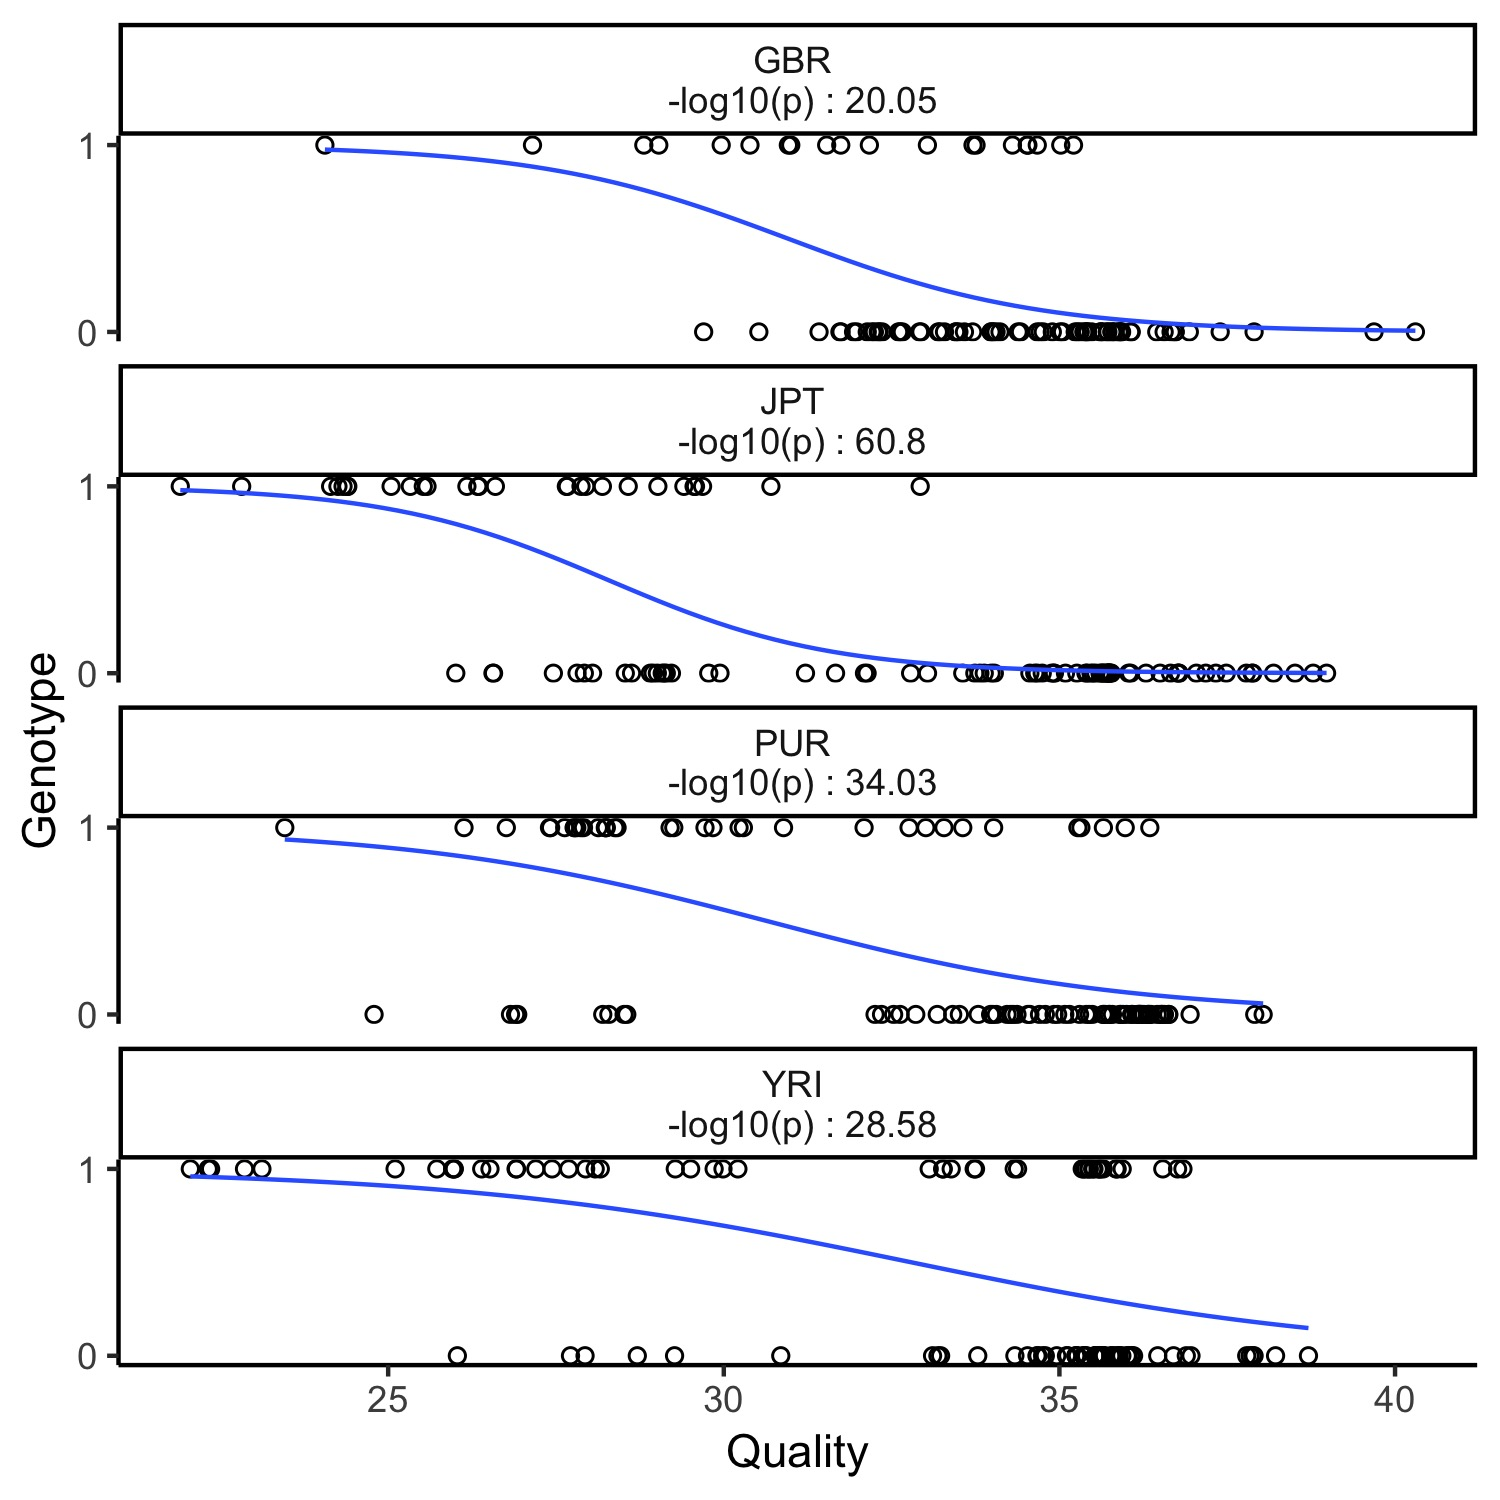
\includegraphics[width=\hsize,keepaspectratio]{./Figures/RegressionPlot.jpg}
\caption{Logistic regression of rs6057648 for the populations with significant association to quality.}
\label{TwinsSNP}
\end{figure}

\begin{figure}
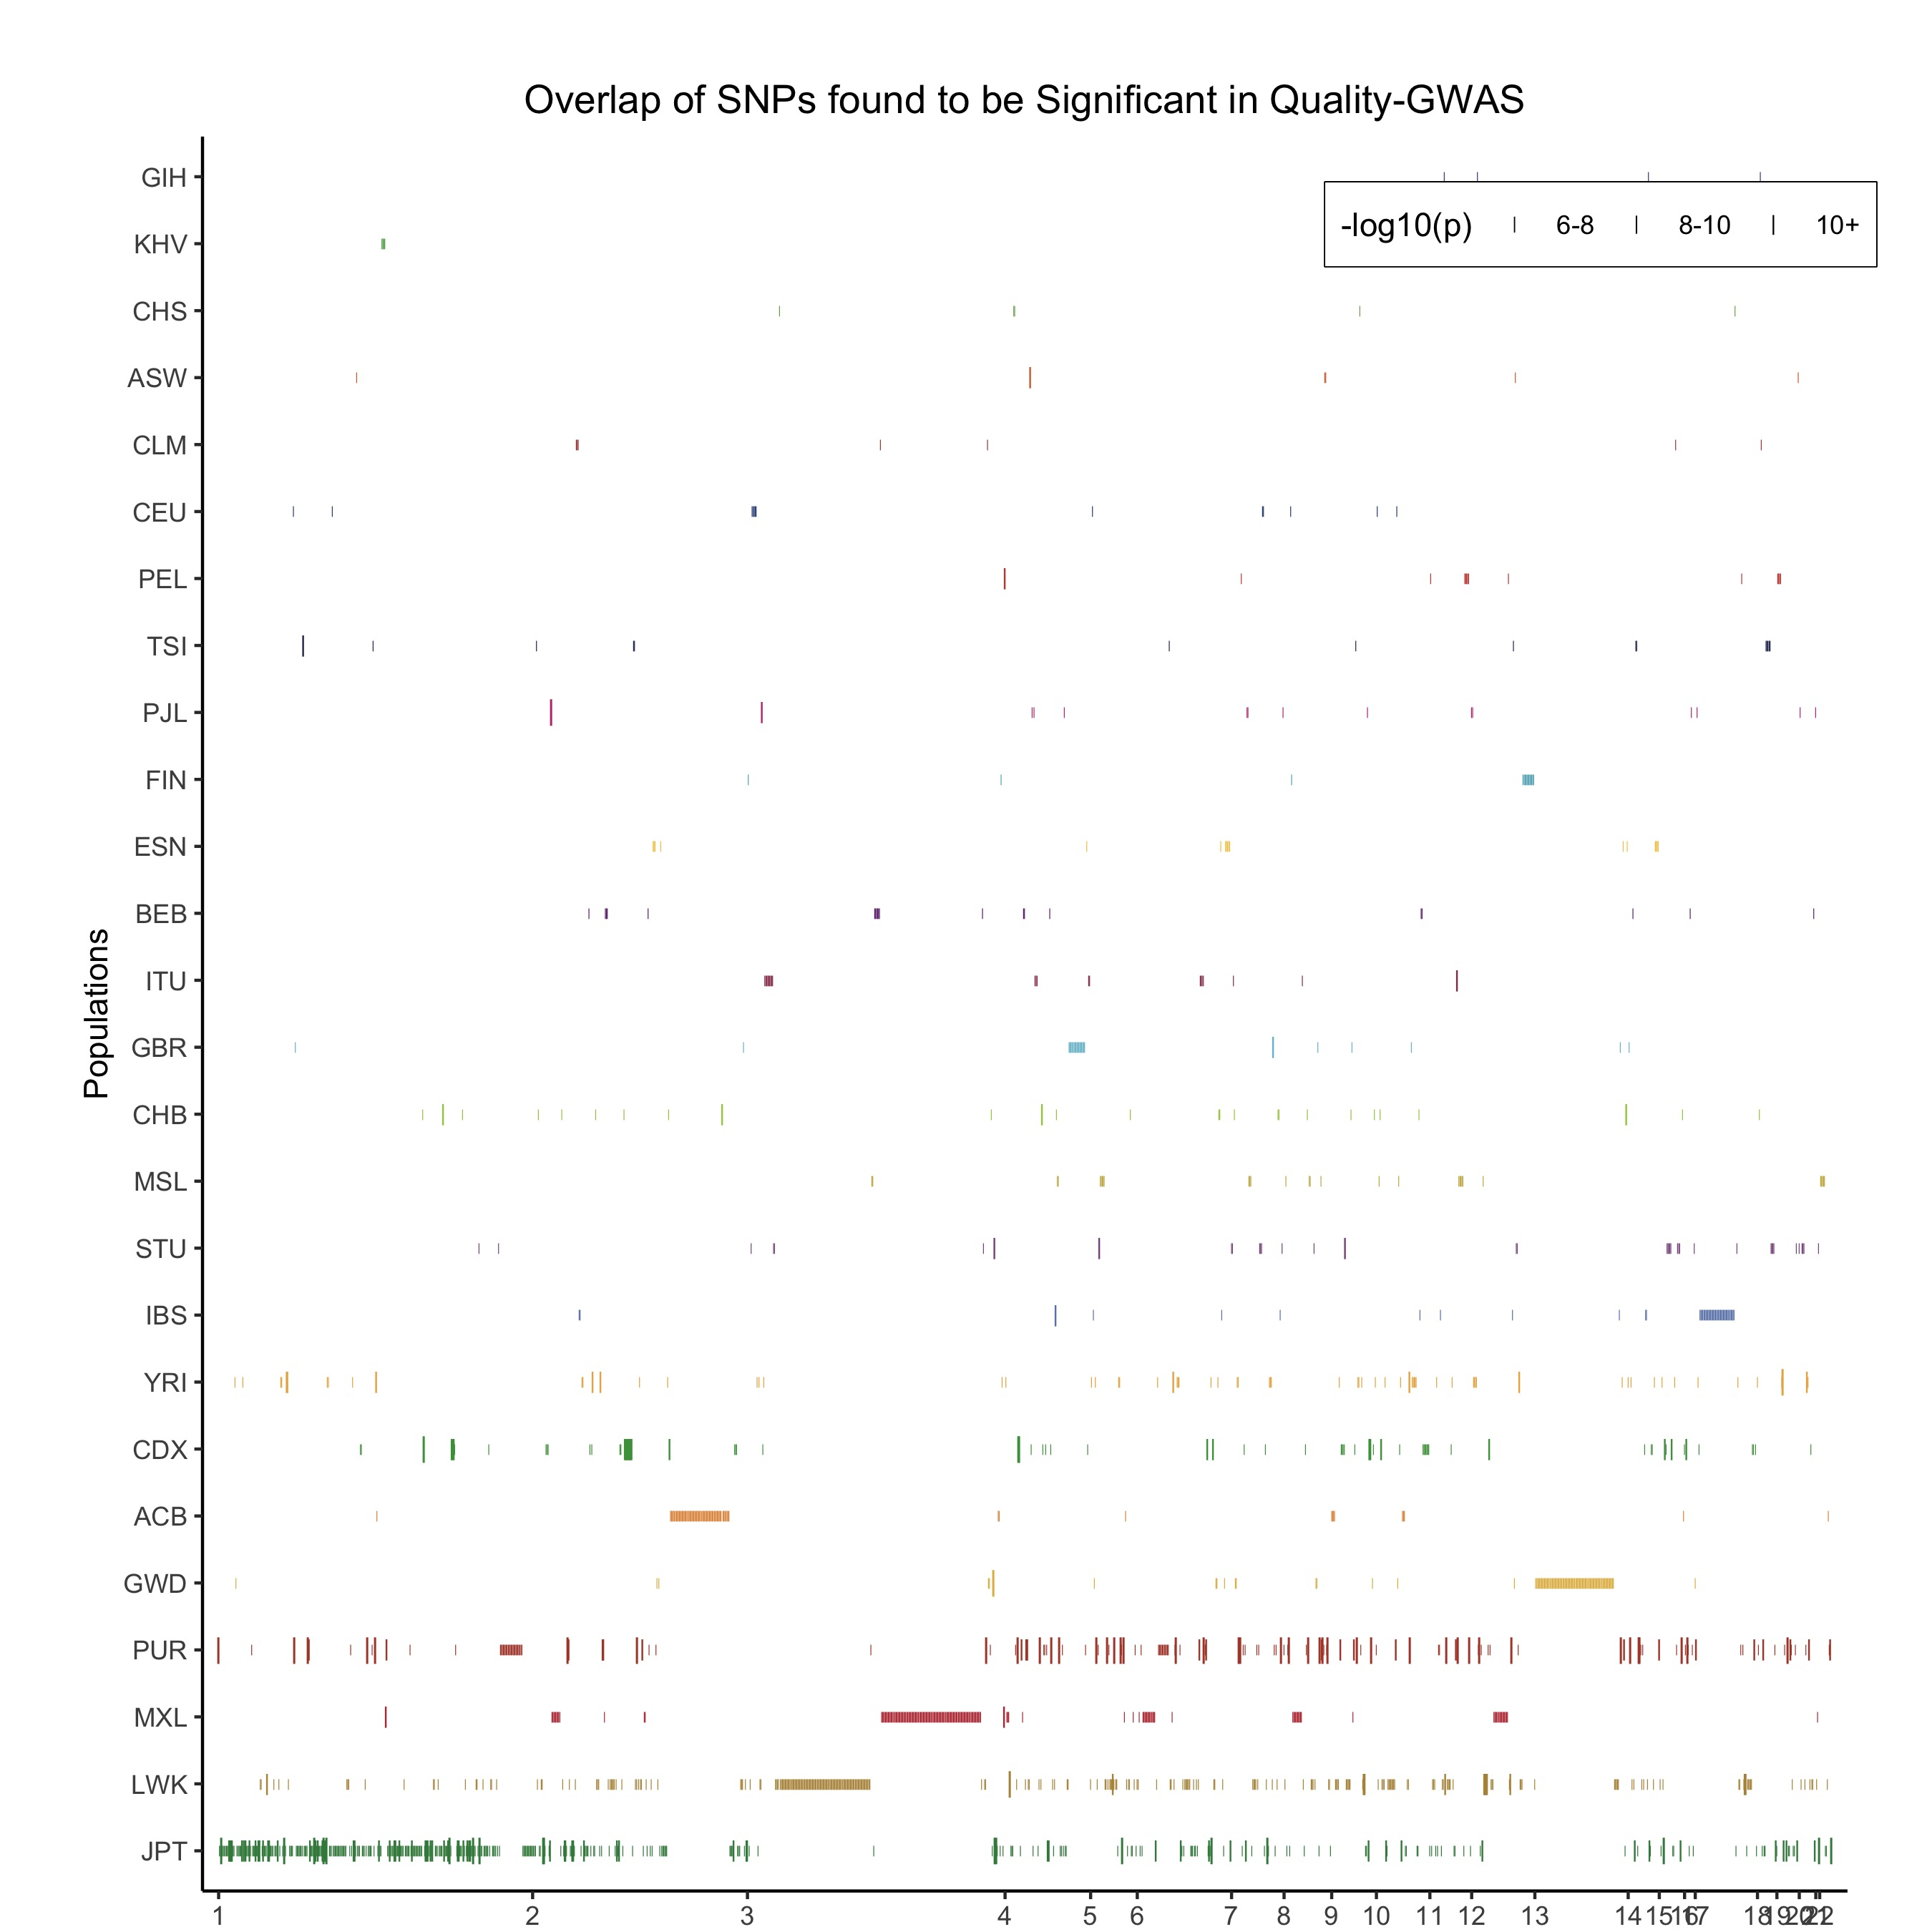
\includegraphics[width=\hsize,keepaspectratio]{./Figures/SNP6_Singles.jpg}
\caption{Significant SNPs found in only one population. The x-axis is sorted by genomic position.}
\label{Singles}
\end{figure}

\end{document}
			
%\begin{center}
 %\begin{tabular}{l l l r r} 
 %\hline
%Author & Year & Journal & RSID & PMID \\ [0.5ex] 
 %\hline
%Ebejer JL	& 2013	 & Twin Res Hum Genet & 	rs6057648&23527680\\ 
 
%Mandage R &	2017	 & PLoS One	 & rs200655768, rs184202621,&28654678\\
%& & & rs201255786, rs201761909&\\
%\hline
%\end{tabular}
%\end{center}